\documentclass[12pt, oneside]{report}   	% use "amsart" instead of "article" for AMSLaTeX format
\usepackage[margin=2.5cm]{geometry}                		% See geometry.pdf to learn the layout options. There are lots.
\geometry{letterpaper}                   		% ... or a4paper or a5paper or ... 
%\geometry{landscape}                		% Activate for rotated page geometry
%\usepackage[parfill]{parskip}    		% Activate to begin paragraphs with an empty line rather than an indent
\usepackage{graphicx}				% Use pdf, png, jpg, or eps§ with pdflatex; use eps in DVI mode
\graphicspath{{./img/}}								% TeX will automatically convert eps --> pdf in pdflatex
					
\usepackage[utf8]{inputenc}
\usepackage[english]{babel}
\usepackage [autostyle, english = american]{csquotes}
\MakeOuterQuote{"}
\usepackage{float}			
\usepackage{lipsum}
\usepackage{amssymb}
\usepackage{amsmath}
\usepackage{amsthm}
\usepackage{mathrsfs}
\usepackage{mathtools}
\usepackage{dsfont}
\usepackage{algorithm}
\usepackage{algpseudocode}
\usepackage[backend=biber, sorting=nty, style=numeric]{biblatex}
\addbibresource{thesis_refs.bib}
%%\usepackage{apacite} %%%
\usepackage{caption}
\usepackage{subcaption}
\usepackage{tcolorbox}
\usepackage{nicematrix}
\usepackage{enumitem}
\usepackage{emptypage}
\usepackage{comment}
\usepackage{setspace}
\usepackage{indentfirst}
\usepackage{systeme}
\usepackage{fancyhdr}
\usepackage{tikz}
\usetikzlibrary{matrix,positioning}
%\usepackage[nottoc,numbib]{tocbibind}
%\usepackage{hyperref}


\newtheorem{theorem}{Theorem}


\DeclareFieldFormat{labelnumberwidth}{\mkbibbrackets{#1}}

\newcommand{\R}{\mathbb{R}}
\newcommand{\C}{\mathbb{C}}
\newcommand{\N}{\mathbb{N}}

\newcommand{\argmax}[1]{\underset{#1}{\operatorname{arg}\,\operatorname{max}}\;}


\newtheorem{defn}{Definition}
\newtheorem{thm}{Theorem}
\newtheorem{lem}{Lemma}
\newtheorem{rmk}{Remark}
\newtheorem{cor}{Corollary}

\DeclarePairedDelimiter{\abs}{\lvert}{\rvert} 
\DeclarePairedDelimiter{\norm}{\lVert}{\rVert}        %norm
\DeclarePairedDelimiter{\inner}{\langle}{\rangle} 
\DeclareMathOperator{\E}{\mathbb{E}}

\DeclareMathOperator{\Adj}{\boldsymbol{A}}
\DeclareMathOperator{\Lplc}{\boldsymbol{L}}
\DeclareMathOperator{\Id}{\boldsymbol{I}}
\DeclareMathOperator{\CC}{\boldsymbol{C}}
\DeclareMathOperator{\MM}{\boldsymbol{M}}
\DeclareMathOperator{\DC}{\boldsymbol{D}(\boldsymbol{C})}
\DeclareMathOperator{\DD}{\boldsymbol{D}}
\DeclareMathOperator{\uu}{\boldsymbol{u}}
\DeclareMathOperator{\uuz}{\boldsymbol{u_0}}
%\DeclareMathOperator{\dot{\uu}}{\boldsymbol{\dot{u}}}
\DeclareMathOperator{\yT}{\boldsymbol{y}(T)}
\DeclareMathOperator{\y}{\boldsymbol{y}}
\DeclareMathOperator{\z}{\boldsymbol{z}}
\DeclareMathOperator{\ytilde}{\boldsymbol{\Tilde{y}}}
\DeclareMathOperator{\vv}{\boldsymbol{v}}
\DeclareMathOperator{\VV}{\boldsymbol{V}}
\DeclareMathOperator{\LLambda}{\boldsymbol{\Lambda}}
\DeclareMathOperator{\UU}{\boldsymbol{U}}

\DeclareMathOperator{\xx}{\boldsymbol{x}}
\DeclareMathOperator{\nuu}{\boldsymbol{\nu}}

%\DeclareMathOperator*{\argmax}{arg\,max}
%\DeclareMathOperator*{\argmin}{arg\,min}
%SetFonts

\makeatletter
\newcommand\frontmatter{%
    \cleardoublepage
 % \@mainmatterfalse
  \pagenumbering{roman}}

\newcommand\mainmatter{%
    \cleardoublepage
%  \@mainmattertrue
  \pagenumbering{arabic}}


\newcommand\backmatter{%
  \if@openright
    \cleardoublepage
  \else
    \clearpage
  \fi
 % \@mainmatterfalse
   }

\makeatother


%SetFonts

%\title{\parbox{\linewidth}{\centering%
%  \textbf{Thesis}\endgraf\bigskip
%  \textbf{Surrogate models for diffusion on graphs: a high-dimensional polynomial approach}\endgraf\bigskip
 % Kylian Ajavon}\endgraf\bigskip
%  Department of Mathematics \& Statistics}
%\author{\parbox{\linewidth}{\centering%
%  Student: Kylian Ajavon\endgraf\medskip
 % Supervisors: Simone Brugiapaglia, Pawel Gora\endgraf}}

%\date{March 2024}
				% Activate to display a given date or no date





\begin{document}

\frontmatter

\begin{titlepage}
\thispagestyle{empty}
\centering
%\vspace*{5cm}
{\Huge\bfseries Surrogate Models for Diffusion on Graphs: A High-Dimensional Polynomial Approach\par}
\vspace{2cm}
{\Large Kylian Ajavon\par}
\vspace{2cm}
{\Large A Thesis in \\
The Department of \\
Mathematics and Statistics\par}
\vspace{2cm}
{\Large Presented in Partial Fulfilment of the Requirements \\
for the Degree of Master of Arts (Mathematics) at \\
Concordia University \\
Montreal, Quebec, Canada\par}
\vfill
{\large March 2024\par}
\vspace{1cm}
\textcopyright \; Kylian Ajavon, 2024
\end{titlepage}

%\clearpage

\begin{comment}
% Signature page
\cleardoublepage % Move to the next page
\thispagestyle{empty} % No headers or footers
%\null\vfil % Vertically center the content on the page
\begin{center}
\textbf{CONCORDIA UNIVERSITY} \\

\textbf{School of Graduate Studies} \\
\end{center}

\vspace{0.5cm}

\noindent This is to certify that the thesis prepared

\vspace{0.5cm}

\noindent By:       Kylian Ajavon 

\vspace{0.5cm}

\noindent Entitled:         Surrogate Models for Diffusion on Graphs: A High-Dimensional Polynomial Approach

\vspace{0.5cm}

\noindent and submitted in partial fulfillment of the requirements for the degree of
\begin{center}
\textbf{Master of Arts (Mathematics)} 
\end{center}

\vspace{0.5cm}

\noindent complies with the regulations of the University and meets the accepted standards with respect to originality and quality.

\vspace{0.5cm}

\noindent Signed by the final Examining Committee:

\vspace{0.5cm}

% Signature part
\begin{flushleft}
\vspace{0.25cm}

\begin{tabular}{@{}p{0.5\textwidth}@{}}
\hline
\centering\textit{} \\
\end{tabular}

\vspace{0.25cm}

\begin{tabular}{@{}p{0.5\textwidth}@{}}
\hline
\centering\textit{} \\
\end{tabular}

\vspace{0.25cm}

\begin{tabular}{@{}p{0.5\textwidth}@{}}
\hline
\centering Dr. Simone Brugiapaglia \\
\end{tabular}

\vspace{0.75cm}

\begin{tabular}{@{}p{0.5\textwidth}@{}}
\hline
\centering Dr. Pawel Góra \\
\end{tabular}
\end{flushleft}

Approved by  \underline{\hspace{8cm}} \\

\vspace{0.75cm}

\hspace{2.5cm} \underline{\hspace{8cm}}\\

\vspace{0.75cm}

Date \underline{\hspace{8cm}}
%\vfil\null
\cleardoublepage % End of the signature page
\end{comment}

\cleardoublepage % Move to the next page
\thispagestyle{empty} % No headers or footers
%\null\vfil % Vertically center the content on the page
\begin{center}
\textbf{CONCORDIA UNIVERSITY} \\

\textbf{School of Graduate Studies} \\
\end{center}

\vspace{0.5cm}

\noindent This is to certify that the thesis prepared

\vspace{0.5cm}

\noindent By:\indent \hspace{\parindent} Kylian Ajavon 

\vspace{0.5cm}

\noindent Entitled: \indent {Surrogate Models for Diffusion on Graphs: A High-Dimensional Polynomial Approach}

\vspace{0.5cm}

\noindent and submitted in partial fulfillment of the requirements for the degree of
\begin{center}
\textbf{Master of Arts (Mathematics)} 
\end{center}

\vspace{0.5cm}

\noindent complies with the regulations of the University and meets the accepted standards with respect to originality and quality.

\vspace{0.5cm}

\noindent Signed by the final Examining Committee:\\

\begin{flushright}
\begin{minipage}{13cm}
\rule{8cm}{0.1mm} Chair and Examiner\vspace{.2cm}\\
Dr. Jason Bramburger\vspace{.2cm}\\
\rule{8cm}{0.1mm} Examiner\vspace{.2cm}\\
Dr. Giuseppe Alessio D'Inverno\vspace{.2cm}\\
\rule{8cm}{0.1mm} Thesis Co-Supervisor\vspace{.2cm}\\
Dr. Simone Brugiapaglia\vspace{.2cm}\\
\rule{8cm}{0.1mm} Thesis Co-Supervisor\vspace{.2cm}\\
Dr. Pawel Góra
\end{minipage}
\end{flushright}
\vspace{.8cm}
Approved by\vspace{-.5cm}
\begin{flushright}
\begin{minipage}{13cm}
\rule{9cm}{0.1mm}
\end{minipage}
\end{flushright}
\vspace{-.7cm} % Reduce the spacing here
\begin{flushright} 
Dr. Lea Popovic, Graduate Program Director
\vspace{.5cm}
\end{flushright}
\begin{flushright}
\begin{minipage}{13cm}
\rule{9cm}{0.1mm} 
\end{minipage}
\end{flushright}
\begin{flushright}
\vspace{-0.3cm}
Dr. Pascale Sicotte, Dean of Faculty of Arts and Science
\end{flushright}
\vspace{.5cm} % Reduce the spacing here
%Date \rule{2.5cm}{0.1mm} 2024\vspace{-.5cm}
Date: \rule{9cm}{0.1mm} 2024



%\maketitle

\begin{abstract}
\thispagestyle{plain}
\setcounter{page}{3}
\begin{center}
Surrogate Models for Diffusion on Graphs: A High-Dimensional Polynomial Approach
\end{center}
\begin{center}
Kylian Ajavon
\end{center}

\vspace{1cm}

\noindent Graphs provide a powerful abstraction for modeling real-world systems, such as social and transportation networks. Of particular significance is the study of diffusion processes on graphs, which is crucial to disciplines spanning biology, engineering and computer science, and to the understanding of phenomena such as disease propagation or the flux of goods and/or people through a transportation network. In this work, we formulate the solution of the diffusion equation on graphs as a parametric model, which gives us insight into the behavior of the diffusion processes by studying how the diffusivity parameters influence the model output. However, accurately simulating the model output of these diffusion processes can be computationally demanding since it involves solving large systems of ordinary differential equations.\\\\
To address this challenge, we propose to construct surrogate models able to approximate the state of a graph at a given time from the knowledge of the diffusivity parameters. In particular, we consider recently introduced techniques from high-dimensional approximation based on sparse polynomial expansions, which are known to produce accurate and sample-efficient approximations when the function to be approximated has holomorphic regularity. Hence, to justify our methodology, we present theoretical results showing that solution maps resulting from a certain class of parametric graph diffusion processes are holomorphic. Then, we demonstrate numerically that it is possible to efficiently compute accurate sparse polynomial surrogate models from a few random samples, hence empirically showing the validity of our approach.

\end{abstract}

\cleardoublepage

\chapter*{Acknowledgements}
\setcounter{page}{4}
%\thispagestyle{empty}

I am immensely grateful to my supervisors, Dr. Simone Brugiapaglia and and Dr. Pawel Góra, for their invaluable support during my studies.\\\\
I would also like to express my sincere appreciation to Dr. Giuseppe Alessio D'Inverno and Dr. Jason Bramburger for their valuable feedback, and to extend my heartfelt thanks again to Dr. Simone Brugiapaglia. Their guidance and advice have been instrumental in shaping my research.\\\\
Finally, I want to voice my deepest thanks to my parents. None of this would have been possible without their unwavering support. Their belief in me has been a source of strength and motivation, and will keep pushing me forward after my studies.

\cleardoublepage

\setcounter{page}{5}
\tableofcontents


\listoffigures
\addcontentsline{toc}{chapter}{List of Figures}

\mainmatter

\chapter{Introduction}
\label{chap:intro}

In the field of applied mathematics, the study of graphs holds significant importance and has widespread applications across numerous disciplines. Their simplicity in abstracting entities as nodes and relationships as edges, enables us to understand and analyze the intricacies of real-world interconnected systems. In particular, the study of diffusion processes on graphs stands as a central component in fields ranging from biology \cite{yi2024graph} to engineering \cite{lejay2003simulating}, and has recently provided major insights in the area of computer science and the development of neural network architectures \cite{chamberlain2021grand}. These diffusion processes, which can describe the spread of diseases \cite{dreyer2009irreversible} or the flow of traffic through a transportation network \cite{barnier2004graph}, are pivotal in understanding and predicting the dynamics of complex networks.\\\\
Central to our work is the approach of formulating the solution of the diffusion equation on graphs as a parametric model, and approximating this model by using polynomials. Parametric models are often used to represent systems, with the aim to understand how the parameters affect the output of the model. These systems are usually complex and can be influenced by many parameters, hence it is not trivial to determine the output of the underlying parametric model. Sometimes, even the value of the parameter is uncertain, which would require the use of stochastic parameterizations and uncertainty quantification \cite{ghanem2017handbook}, in order to estimate and quantify the uncertainty in the output. Moreover, it is typically expensive to evaluate the output of a parametric model, making it challenging to perform parametric studies on the model. For that reason, it is often desirable to construct a surrogate model from sample values, to approximate the parametric model. For example, techniques such as reduced basis method \cite{negri2013reduced} have been used to build efficient surrogate models for parametric partial differential equations. In our case, we use methods from the discipline of high-dimensional polynomial approximation, which gives us a solid mathematical framework for tackling the challenges posed by the complex and high-dimensional nature of graph-based systems.\\\\
We begin this thesis with an overview of graph theory. In Chapter \ref{chap:graphs}, we introduce basic graph theory concepts that are relevant to our research objectives. In particular, we examine diffusion processes on graphs and the differential equations associated with these processes. We also review numerical methods for solving differential equations. Following that, in Chapter \ref{chap:functions}, is a study of the relevant mathematical background on high-dimensional polynomial approximation. We present concepts from polynomial approximation theory, starting with one-dimensional functions before extending the idea to multiple dimensions. We also discuss sparsity in relation to polynomial approximation. We then have a more detailed discussion on parametric models and the idea of approximating a parametric solution map via a surrogate model. We conclude the chapter by reviewing why holomorphic functions have desirable properties in the context of sparse polynomial approximation. In chapter \ref{chap:research}, we introduce our formulation of the diffusion equation on graphs as a parametric model, and we provide novel theoretical results with regards to the validity of our approach. In particular, Theorem \ref{thm:mainthm} presents results on the holomorphic regularity of our surrogate model, showing that we can efficiently compute accurate sparse polynomial surrogate models of the diffusion equation on graphs. These theoretical results are then supported by various numerical experiments. Finally, in Chapter \ref{chap:conclusion}, we discuss the implications of our findings, and the limitations of our approach, highlighting potential applications and direction for future research.



\newpage


\chapter{Theoretical background on graphs}
\label{chap:graphs}

In this chapter we establish the theoretical background on graphs that will be needed for this research. In Section \ref{sec:graphs}, we define a graph as a mathematical object, as well as some common graph representation matrices such as the graph Laplacian. Additionally, we review some properties of the latter which will be of interest to us. We also discuss random graphs: in particular, we introduce generative models such as stochastic block models, which provide us with the appropriate graph structure for our problem.\\
In Section \ref{sec:diffusion} we focus on diffusion processes on graphs. We introduce the diffusion equation and derive an explicit solution for its simplest form. We also propose two variants of the diffusion equation, that will be the focus of this work.\\
Finally, Section \ref{sec:num_methods} is centered around numerical integration techniques to solve ordinary differential equations. We give a brief introduction of a few methods, which will be applied to solve the diffusion equation on graphs, and its variants presented in Section \ref{sec:diffusion}.\\\\
\textbf{Relevant literature}\\\\
For further reading on graph theory concepts, see \cite{gross2018graph, Newman2010}. In particular, \cite{Newman2010} focuses more on concepts related to diffusion processes on graphs. Random graphs and select models are discussed further in \cite{bollobas1998random, erdds1959random, holland1983stochastic}. Finally, for more information on numerical methods for ordinary differential equations, see \cite{burden2010numerical, butcher2016numerical, dormand1980family, bogacki19893, shampine1986some}.


\section{Graphs}
\label{sec:graphs}

% What is a graph
% how to represent graph (adjacency matrix)
% other important statistics/metrics to represent graphs (degree, etc)
% briefly mention Laplacian
% stochastic block models..?

In this section, we first define graphs in a mathematical framework and introduce basic graph theory concepts. We then define random graph generative models, and present a model that will be used for our numerical experiments.

\subsection{Basic graph theory concepts}

A graph $\mathcal{G}=(\mathcal{V}, \mathcal{E})$ is a mathematical object composed of a set of nodes (or vertices) $\mathcal{V}$ and a set of edges $\mathcal{E}$. An edge connecting two nodes $u,v\in\mathcal{V}$ is denoted as a couple $(u,v)\in\mathcal{E}$. Graphs are a versatile data structure, as they can be used to represent any system where components interact with each other, or entities with relationships between them.\\\\
There are several ways to represent a graph in order to perform operations related to a given graph. The most commonly used representation is the \textbf{adjacency matrix}. The entries $A_{ij}$ of the adjacency matrix $\boldsymbol{A}$ for a graph $\mathcal{G}=(\mathcal{V}, \mathcal{E})$ are defined as:

\begin{equation*}
A_{ij}=
    \begin{cases}
        1 & \text{if } (i,j)\in\mathcal{E}\\
        0 & \text{if } (i,j)\notin\mathcal{E}
    \end{cases}.
\end{equation*}\\\\
Note that in this work, we only consider \textbf{undirected and unweighted graphs}, i.e., graphs where all the edges are bidirectional and where the edges do note have any weights associated to them. Formally, for two nodes $i$ and $j$ in an undirected graph, if $(i,j)\in\mathcal{E}$, then $(j,i)\in\mathcal{E}$. For this reason, the adjacency matrix of an undirected graph is symmetric. As an illustration, Figure \ref{fig:graph_adjacency} shows an example of a graph with its corresponding adjacency matrix.
\begin{figure}[t]
  \centering
  \begin{minipage}{0.45\textwidth}
    % Graph
    \begin{center}
      \begin{tabular}{c}
        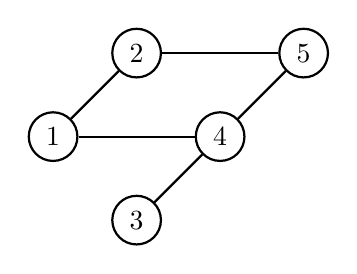
\begin{tikzpicture}[node distance={15mm}, thick, main/.style = {draw, circle}] 
          % Define nodes
          \node[main] (1) {1}; 
          \node[main] (2) [above right of=1] {2}; 
          \node[main] (3) [below right of=1] {3}; 
          \node[main] (4) [above right of=3] {4}; 
          \node[main] (5) [above right of=4] {5};
          % Add edges
          \draw (1) -- (2);
          \draw (1) -- (4);
          \draw (2) -- (5);
          \draw (3) -- (4);
          \draw (4) -- (5);
        \end{tikzpicture}
      \end{tabular}
    \end{center}
  \end{minipage}
  %\hspace{1cm}
  \begin{minipage}{0.45\textwidth}
    % Adjacency Matrix
    \begin{center}
      \[
        \begin{bmatrix}
          0 & 1 & 0 & 1 & 0 \\
          1 & 0 & 0 & 0 & 1 \\
          0 & 0 & 0 & 1 & 0 \\
          1 & 0 & 1 & 0 & 1 \\
          0 & 1 & 0 & 1 & 0 \\
        \end{bmatrix}
      \]
    \end{center}
  \end{minipage}
  \caption{Graph and corresponding adjacency matrix}
  \label{fig:graph_adjacency}
\end{figure}
We can also have a better understanding of graphs with some important graph statistics, such as the \textbf{degree} of a node. The degree of a node $u$, which we will denote $\deg(u)$, refers to the number of nodes that are connected to node $u$ by an edge. Equivalently, in an undirected graph, the degree of a node can be defined as the sum of the entries of the corresponding row in the adjacency matrix:
$$
\deg(i)=\sum_{j\in\mathcal{V}} A_{ij}.
$$
This could give us an idea of how important a specific node is within a given graph. The \textbf{degree matrix} $\boldsymbol{D}$ of a graph is a diagonal matrix, where 
\begin{equation}
\label{eq:degree}
D_{ii}=\deg(i).
\end{equation}
\noindent Another way to represent a graph is by using the \textbf{graph Laplacian} $\boldsymbol{L}$ (or the Laplacian matrix), defined as
\begin{equation}
\boldsymbol{L}=\boldsymbol{D}-\boldsymbol{A}.
\end{equation} 
This matrix encodes the connections of all the nodes in the graph, but also how connected each node is to the other nodes in the graph. It is especially important for problems involving diffusion processes on graphs, which we will cover in more detail in the next subsection. 
\begin{rmk}
\label{rmk:lplc_properties}
The graph Laplacian has a few properties that will be of interest to us. Firstly, a Laplacian matrix $\Lplc$ is positive-semidefinite \cite{Newman2010}. In other words, all of its eigenvalues are nonnegative. Furthermore, the sum of the rows (or the columns) of $\Lplc$ equals 0. Consequently, the smallest eigenvalue $\lambda_1=0$ and its corresponding eigenvector is $\boldsymbol{v}_1=(1,1,...,1)^T$.
\end{rmk}

\subsection{Random graphs and stochastic block models}

In practice, we will be using generative models to solve our graph-related problems, by using \textbf{random graphs} \cite{bollobas1998random}. A random graph is a model for a graph where edges are added between nodes, following a given probability distribution. The most commonly used random graph model is the Erdös-Renyi model \cite{erdds1959random}, which actually has two variants: the $G(n,M)$ model (which randomly chooses a graph in the collection of all graphs with $n$ nodes and $M$ edges), and the $G(n,p)$ model (which constructs a graph with $n$ nodes and includes an edge between a pair of nodes, with probability $p$). In this work, we will be interested in graphs with a community structure, where the edge "within-group" density is high, and the edge "between-group" density is low. Here, the edge density is informally understood as the ratio between the number of edges within a community $\mathcal{C}_k$ and all the possible pairs $(i,j)$ for nodes $i,j\in\mathcal{C}_k$.
\begin{figure}[t]
\centering
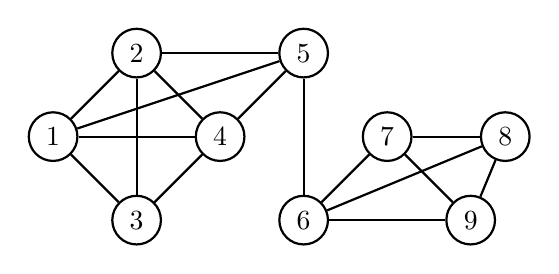
\begin{tikzpicture}[node distance={15mm}, thick, main/.style = {draw, circle}] 
\node[main] (1) {1}; 
\node[main] (2) [above right of=1] {2}; 
\node[main] (3) [below right of=1] {3}; 
\node[main] (4) [above right of=3] {4}; 
\node[main] (5) [above right of=4] {5}; 
\node[main] (6) [below right of=4] {6}; 
\node[main] (7) [above right of=6] {7}; 
\node[main] (8) [right of=7] {8}; 
\node[main] (9) [below right of=7] {9}; 
\draw (1) -- (2); 
\draw (1) -- (3);
\draw (1) -- (4);
\draw (1) -- (5);
\draw (2) -- (3);
\draw (2) -- (4);
\draw (2) -- (5);
\draw (3) -- (4); 
\draw (5) -- (4);
\draw (6) -- (7);
\draw (6) -- (8);
\draw (6) -- (9);
\draw (8) -- (7);
\draw (9) -- (7);
\draw (8) -- (9); 
\draw (5) -- (6); 
\end{tikzpicture}
\caption{Example of a graph with community structure}
\label{fig:graph_comm}
\end{figure}
\noindent The example in Figure \ref{fig:graph_comm} showcases a graph with 2 communities $C_1=\{1,2,3,4,5\}$ and $C_2=\{6,7,8,9\}$, where the edge density is high within $C_1$ and $C_2$, while it is low between the two communities, as the only edge connecting them is the edge $(5,6)$.\\\\
A more appropriate random graph model which captures that community structure is the \textbf{stochastic block model} (or \textbf{SBM}) \cite{holland1983stochastic}. The SBM is a generative model that takes three parameters:
\begin{itemize}
    \item $n$: the number of nodes,
    \item $\alpha_r$: a partition of $r$ disjoint subsets of the vertex set $\{1,...,n\}$,
    \item $\boldsymbol{P}\in[0,1]^{r\times r}$: a matrix of edge probabilities,
\end{itemize}
and constructs a graph such that the distribution of the edges between nodes is dependent on the communities to which the nodes belong \cite{holland1983stochastic}. The edge probabilities $P_{ij}$ can be chosen such that the resulting graph matches our desired setup: this could be achieved by choosing a diagonally dominant matrix $\boldsymbol{P}$, i.e., the magnitude of the diagonal entry in a row of $\boldsymbol{P}$ is larger than or equal to the sum of the magnitudes of all the non-diagonal entries in that row.
\begin{figure}[t]
    \centering
    \includegraphics[scale=0.4]{sbmexample.png}
    \caption{Example of a graph generated with a stochastic block model}
    \label{fig:example_sbm}
\end{figure}
\noindent In Figure \ref{fig:example_sbm}, we show an example of a graph generated from a SBM with $n=15$, $\alpha_r=\{\{0,1,2,3,4,5\}, \{6,7,8,9,10\}, \{11,12,13,14\}\}$ and 
$$
 \boldsymbol{P} =
\begin{bmatrix}
1 & 0.05 & 0.05 \\
0.05 & 1 & 0.05 \\
0.05 & 0.05 & 1 \\
\end{bmatrix}.
$$
\noindent The Erdös-Renyi $G(n,p)$ model is a special case of that model, as it is equivalent to the SBM with $\alpha_r=\{1,2,...,n\}$ and $P_{ij}=p$ for all $i,j$. Given its ability to produce graphs with communities, the stochastic block model is often used in modeling social networks \cite{holland1983stochastic}, biological networks \cite{morelli2021nested}, citation networks \cite{hric2018stochastic}, etc.



\section{Diffusion on graphs}
\label{sec:diffusion}

% talk about diffusion processes and why it might be interesting
% derive Newman equation
% derive solution

There are different types of diffusion processes. For instance, information in a social network does not necessarily propagate in the same way heat does on a surface. One could consider diffusion processes modelled by random walks \cite{blum2020foundations}, where a particle circulates randomly along the edges of a graph, or modelled by differential equations. In this research, we consider the latter. The diffusion processes we are interested in can be considered as the discrete analogy to the diffusion of heat on a continuous domain.\\\\
We want to be able to denote the quantity of a “substance” at each node $i$ in a graph, and how that quantity evolves as time progresses. We can denote this quantity by using a vector-valued function $\uu(t)$. The quantity at each node $i$ is then denoted as $u_i(t)$ (or $u_i$). As outlined in \cite{Newman2010}, suppose the substance is flowing from node $j$ to node $i$ at a rate $C(u_j - u_i)$ (assuming the nodes $i$ and $j$ are connected by an edge), where $C$ is called the \textbf{diffusion constant}. Hence, the rate of change of $u_i$ is given by
$$
\dot{\uu}_i = C\sum_{j\in\mathcal{V}} A_{ij}(u_j - u_i).
$$
In other words, the change in the quantity of the substance at node $i$ is equal to the sum of the changes in quantity in all the nodes adjacent to node $i$. Note that for simplicity, we will sometimes denote $\uu(t)$ as $\uu$ and $\dot{\uu}(t)$ as $\dot{\uu}$. Hence, we have
\begin{align*}
\dot{\uu}_i &= C\sum_{j\in\mathcal{V}} \Adj_{ij}u_j - C\sum_{j\in\mathcal{V}} \Adj_{ij}u_i \\
 &= C\sum_{j\in\mathcal{V}} \Adj_{ij}u_j - Cu_i\sum_{j\in\mathcal{V}} \Adj_{ij} \\
 &= C\sum_{j\in\mathcal{V}} \Adj_{ij}u_j - Cu_i\deg(i) \\
 &= C\sum_{j\in\mathcal{V}} \Adj_{ij}u_j - u_i\deg(i) \\
 &= C\sum_{j\in\mathcal{V}} (\Adj_{ij} - \delta_{ij}\deg(i))u_j,
\end{align*}
where the \textbf{Kronecker delta} is defined as $\delta_{ij}=1$ if $i=j$, or $\delta_{ij}=0$ otherwise. In matrix form, we get
$$
\dot{\uu} = C(\Adj - \DD)\uu.
$$
As a result, we obtain the following \textbf{diffusion equation}
\begin{equation}
\label{eq:diff}
\dot{\uu}(t) = -C\Lplc\uu(t).
\end{equation}
The solution can be derived in a few steps.
\begin{align*}
\dot{\uu} &= -C\Lplc\uu \\
\dot{\uu} &= -C\VV\LLambda\VV^*\uu && \text{(after diagonalizing $\Lplc=\VV\LLambda\VV^*$)} \\
\VV^*\dot{\uu} &= -C\LLambda\VV^*\uu && \text{(since $\VV^*\VV=\Id$)} \\
(\dot{\boldsymbol{V^*u}}) &= -C\LLambda(\VV^*\uu)
\end{align*}
Note that the steps above work by applying the spectral theorem, thanks to the symmetry of $\Lplc$ (as mentioned in Remark \ref{rmk:lplc_properties}). Let $\boldsymbol{a}=\VV^*\uu$. With this change of variable, we obtain the equation
$$
\boldsymbol{\dot{a}} = -C\LLambda\boldsymbol{a}.
$$
Since $\LLambda$ is a diagonal matrix, this system of ordinary differential equations is separable and can be expressed as 
$$
\dot{a}_i = -C\lambda_i a_i \quad \forall i\in\mathcal{V}.
$$
This is a first order homogeneous linear differential equation, which is solved by
$$
a_i(t) = a_i(0)e^{-C\lambda_i t} \quad \forall i\in\mathcal{V}.
$$
Since $\uu=\VV\boldsymbol{a}$, the solution $\uu(t)$ is given by a linear combination of the eigenvectors $\vv_i$ of $\Lplc$:
$$
\uu(t) = \sum_{i\in\mathcal{V}} a_i(t) \vv_i.
$$
The properties of $\Lplc$ give us some insights into the "mechanics" of $\uu(t)$. Recall from Remark \ref{rmk:lplc_properties} that the eigenvalues of the graph Laplacian $\Lplc$ are all nonnegative, the smallest eigenvalue is $\lambda_1=0$ and its corresponding eigenvector is $\boldsymbol{v}_1=(1,1,...,1)$. By looking more closely at $\uu(t)$, we get:
\begin{align*}
\uu(t) &= \sum_{i\in\mathcal{V}} a_i(t) \vv_i \\
&= \sum_{i\in\mathcal{V}} a_i(0)e^{-C\lambda_i t} \vv_i \\
&= a_1(0)e^{-C\lambda_1 t} \vv_1 + a_2(0)e^{-C\lambda_2 t} \vv_2 + ... + a_n(0)e^{-C\lambda_n t} \vv_n \\
&= a_1(0)\vv_1 + a_2(0)e^{-C\lambda_2 t} \vv_2 + ... + a_n(0)e^{-C\lambda_n t} \vv_n,
\end{align*}
where $0\leq\lambda_2\leq...\leq\lambda_n$. Consequently, as $t$ increases, $e^{-C\lambda_i t}\rightarrow0$ for $i$ such that $\lambda_i=0$, or equivalently $\uu(t)\rightarrow \alpha \cdot(1,1,...,1)$, where $\alpha=\sum_{i\in\mathcal{V}}a_i(0)$ for $i$ such that $\lambda_i=0$. This makes sense intuitively, if we consider how heat propagates on a surface. Given some initial condition (with some regions of the surface being hotter than other regions), as time progresses, the temperature in all the regions of the surface reaches an equilibrium. This is what happens in our case because as time progresses, all the nodes in the graph end up having the same quantity, as illustrated in Figure \ref{fig:diff_snapshots}.
\begin{figure}[t]
    \centering
    \includegraphics[width=\textwidth]{diff_progression.png}
    \caption{Snapshots of $\uu(t)$ for a given graph, for a constant, uniform diffusion process with $C=2$}
    \label{fig:diff_snapshots}
\end{figure}
\noindent Recall that in equation \eqref{eq:diff}, the constant $C$ implies that the diffusion process is uniform (invariant for all edges) and constant (invariant with respect to time) along the edges of the graph. In this work, we consider the case where instead of only one diffusion constant $C$, we assign new diffusion constants $C_{ij}$ for each edge $(i,j)$. The literature on non-constant diffusion processes modelled by differential equations on graphs is scarce, but we can derive an equation for edge-dependent diffusion on a graph, similar to equation \eqref{eq:diff}. We start from
\[\dot{u_i}(t) = C \sum_{j\in\mathcal{V}} A_{ij}(u_j(t) - u_i(t)), \quad i\in\mathcal{V}\]
We can assign new edge-dependent diffusion parameters $C_{ij}$ to obtain the following diffusion equation, for any $i\in\mathcal{V}$
\begin{align*}
\dot{u_i} &= \sum_{j\in\mathcal{V}} C_{ij} A_{ij}(u_j - u_i) \\
&= \sum_{j\in\mathcal{V}} C_{ij} A_{ij}u_j - u_i \sum_{j\in\mathcal{V}} C_{ij} A_{ij} \\
&= \sum_{j\in\mathcal{V}} \left[C_{ij} A_{ij} - \delta_{ij}\left(\sum_{k\in\mathcal{V}} C_{ik} A_{ik}\right)\right] u_j \\
&= \left[(\CC \odot \Adj - \DC)\uu(t)\right]_i
\end{align*}
where $D_{ij}(\CC) = \delta_{ij}\sum_k C_{ik} A_{ik}$, and $\odot$ denotes the \textbf{Hadamard product} (or entrywise product) of two matrices, defined as $(\boldsymbol{X}\odot\boldsymbol{Y})_{ij}=X_{ij}Y_{ij}$. The equation for edge-dependent diffusion on a graph can thus be rewritten as
\begin{equation}
\label{eq:nonconstant}
\dot{\uu}(t)=\MM\uu(t),
\end{equation}
where $\MM=\CC\odot\Adj-\DC$.
\begin{rmk}
\label{rmk:weightedlap}
Note that in equation \eqref{eq:nonconstant}, the matrix $\MM$ is equivalent to a weighted Laplacian matrix $\Lplc=\DD-\boldsymbol{W}$, where $\boldsymbol{W}$ is a weighted adjacency matrix defined by 
$$
W_{ij} = 
    \begin{cases}
        s(i,j) & \text{if } (i,j)\in\mathcal{E}\\
        0 & \text{if } (i,j)\notin\mathcal{E}
    \end{cases},
$$
$s(i,j)$ denoting the weight of the edge connecting nodes $i$ and $j$, and where $\DD$ is a weighted degree matrix defined by $D_{ii}=\sum_{j\in\mathcal{V}}W_{ij}$ \cite{foucart2022mathematical}.
\end{rmk}

\noindent We can make further modifications to have a more generalized setup. On top of applying new diffusion coefficients $C_{ij}$ to our graph, let us consider those diffusion coefficients to be time-dependent. In other words, we assign new diffusion coefficients $C_{ij}(t)$ for each edge $(i,j)$. The derivation of the diffusion equation corresponding to this problem is identical to the one above, and we obtain the following equation:
\begin{equation}
\label{eq:nonconstanttime}
\dot{\uu}(t)=\MM(t)\uu(t),
\end{equation}
where $\MM(t)=\CC(t)\odot\Adj-\boldsymbol{D}(\CC(t))$. This edge-and-time-dependent diffusion equation is no longer solvable analytically, unless the time dependency is asymptotically constant or periodic \cite{floquet1883equations}. Therefore we have to use numerical integration techniques to find an approximation for $\uu(t)$.

\section{Numerical methods for graph diffusion}
\label{sec:num_methods}

This subsection is about the different techniques we can use to find an approximation to the solution of our diffusion ODE. Recall that
$$
\dot{\uu}(t) = \MM(t)\uu(t), \quad \uu(t_0)=\uu_0
$$
This is a first-order initial value problem (IVP), which can be solved with traditional numerical methods. 
%In particular, we want to consider methods that are efficient at solving stiff ODEs. Informally, a stiff ODE is a type of ODE where the solution has wildly varying timescales. Our equation equation \eqref{eq:nonconstanttime} is not stiff by default, however this could depend on our choices for the time dependencies of the diffusion. For instance, ...\\\\
%In this work, we will consider two numerical methods: the \textbf{backward Euler} method (BE) and the \textbf{fourth-order Runge-Kutta} method (RK4).
There are numerous methods to solve IVPs, and they are not necessarily graph-related, as we are dealing with a simple system of first-order ordinary differential equations. Such methods includes the Euler method, the Runge-Kutta methods and linear multistep methods like the Adams-Moulton or the Adams-Bashforth methods \cite{burden2010numerical, butcher2016numerical}.\\\\ 
%There are a few properties to consider when choosing an appropriate numerical method \cite{burden2010numerical}:
\iffalse
\begin{itemize}
    \item \textbf{stability}: a stable numerical method is a method that produces bounded solutions over long time periods or with larger step sizes. 
    \item \textbf{convergence}: an appropriate numerical method should be convergent, i.e., the approximation obtained from the method should approach the exact solution of the ODE, as the step size decreases. An even more desirable property would be strong convergence, which refers to when the error between the numerical solution and the exact solution decreases at a rate faster than the step size.
    \item \textbf{accuracy}: an accurate method should produce solutions that do not deviate too much from the exact solution. The error between the numerical solution and the exact solution should be sufficiently small.
    \item \textbf{order}: the order of a numerical method refers to the rate at which the error decreases as the step size decreases.
    \item \textbf{efficiency}: it is also desirable for a numerical method to be computationally efficient. In other words, the method should require minimum computational resources (time and memory). This becomes more important as we increase the dimension of our problem. However, one thing to keep in mind is that there is usually a trade-off between efficiency and accuracy.
\end{itemize}
\fi
In this work, we will only consider the following methods: the \textbf{forward Euler} method, the \textbf{backward Euler} method and the \textbf{Runge-Kutta} methods. We will compare the numerical performance of these methods in Section \ref{sec:numerics}.

\subsection{Forward Euler}

The forward (or explicit) Euler method, is a simple first-order explicit method that approximates the solution of an ODE at the next time step based on the current value and the derivative at the current time step. The method can be derived by using the forward finite differences to approximate the derivative, i.e., 
$$
\dot{\uu}(t) \approx \frac{\uu(t+h)-\uu(t)}{h},
$$
where $h>0$ is the step size. From equation \eqref{eq:nonconstanttime}, it follows that
\begin{align*}
\MM(t)\uu(t) &= \frac{\uu(t+h)-\uu(t)}{h} \\
h\MM(t)\uu(t) &= \uu(t+h)-\uu(t) \\
\uu(t+h) &= \uu(t) + h\MM(t)\uu(t) \\
\uu(t+h) &= (\Id + h\MM(t))\uu(t).
\end{align*}
Thus, we obtain the following update rule:
\begin{equation}
\uu^{(k+1)} = [\Id + h\MM(t_k)]\uu^{(k)},
\end{equation}
where $t_k = t_0+kh$ and $\uu^{(k)}$ is an approximation for $\uu(t_k)$ for $k=0,1,2,...$.\\\\
We define the order of accuracy of a numerical method as the rate of convergence of a numerical solution to the exact solution of a differential equation, i.e., for a given step size $h$, a numerical method is $n^{th}$-order accurate if the error is roughly proportional to $h^n$ \cite{leveque2007finite}.\\\\
\iffalse
\begin{defn}[Order of accuracy]
Let $u(t)$ be the exact solution to a differential equation, and let $u(t)_h$ be a numerical approximation of $u(t)$ given some step size $h$. The numerical solution $u(t)_h$ is $n^{th}$-order accurate if the error is roughly proportional to $h^n$. In other words,
$$
\norm{\uu-\uu_h}\leq Ch^n
$$
for some constant $C$.
\end{defn}
\fi
\noindent The forward Euler method is first-order accurate. It is also simple to implement and computationally efficient.

\subsection{Backward Euler}

The backward Euler method is an implicit first-order method: unlike the forward Euler method, it uses information from the current time step and the previous time step to approximate the solution at the next time step. The method is derived by using the backward finite differences to approximate the derivative, i.e.,
$$
\dot{\uu}(t)\approx\frac{\uu(t)-\uu(t-h)}{h}.
$$
Similarly to the forward Euler method, we can use equation \eqref{eq:nonconstanttime} to derive the following:
\begin{align*}
\MM(t)\uu(t) &= \frac{\uu(t)-\uu(t-h)}{h} \\
h \MM(t)\uu(t) &= \uu(t)-\uu(t-h) \\
\uu(t) - h \MM(t)\uu(t) &= \uu(t-h) \\
(\Id - h \MM(t))\uu(t) &= \uu(t-h) \\
\uu(t) &= (\Id - h \MM(t))^{-1}\uu(t-h).
\end{align*}
This gives us the update rule
\begin{equation}
\uu^{(k+1)} = [\Id - h\MM(t_{k+1})]^{-1}\uu^{(k)}.
\end{equation}
%In our problem, using the BE method has a few advantages. Firstly, it is unconditionally stable for linear ODEs, i.e. the numerical solution approaches the true solution as $h$ approaches zero. This method is also effective for solving stiff ODEs.
The backward Euler method is also first-order accurate in time. Since it is an implicit method, it can be more computationally expensive than the forward Euler method. One advantage this method does offer is that it is generally more stable and more accurate than the forward Euler method \cite{quarteroni2006scientific}.

\subsection{Runge-Kutta methods}

%The RK4 method is a multistep method that, similarly to the BE method, gives an approximation for $\uu(t)$ by iterating for some $k$ such that $\uu^{(k)}\rightarrow\uu(t)$. The main difference in the approach is that instead of taking one previous point and its derivative to determine the current value of $\uu(t)$, we take intermediate steps to obtain a more accurate approximation. We get the following iterations, for $k=0,1,2,...$
The Runge-Kutta methods refer to a family of methods based on weighted averages of multiple function evaluations. Essentially, as opposed to the forward and backward Euler methods which approximate the solution by taking a single step forward in time, the Runge-Kutta methods use intermediate steps before approximating the next time step of the solution. This is done to achieve a higher-order accuracy compared to the Euler methods.\\\\
There exist different variants of the Runge-Kutta method, and the differences between them lie in the number of stages in the method, as well as the coefficients used to compute the weighted averages. One of the most commonly known and used variants is the \textbf{fourth-order Runge-Kutta} method (or RK4), which has the following update rule:
\begin{align*}
\boldsymbol{k}_1^{(k+1)} &= \MM(t_k)\uu^{(k)} \\
\boldsymbol{k}_2^{(k+1)} &= \MM(t_k+\frac{h}{2})[\uu^{(k)}+\frac{h}{2}\boldsymbol{k}_1^{(k+1)}] \\
\boldsymbol{k}_3^{(k+1)} &= \MM(t_k+\frac{h}{2})[\uu^{(k)}+\frac{h}{2}\boldsymbol{k}_2^{(k+1)}] \\
\boldsymbol{k}_4^{(k+1)} &= \MM(t_k+h)[\uu^{(k)}+h\boldsymbol{k}_3^{(k+1)}] \\
\uu^{(k+1)} &= \uu^{(k)} + \frac{h}{6}(\boldsymbol{k}_1^{(k+1)} + 2\boldsymbol{k}_2^{(k+1)} + 2\boldsymbol{k}_3^{(k+1)} + \boldsymbol{k}_4^{(k+1)})
\end{align*}
There also exist higher-order variants, such as RK45 or RK23 \cite{dormand1980family, shampine1986some, bogacki19893}.\\\\
The Runge-Kutta methods offer a better accuracy than the forward and backward Euler methods, for a given $h$ (provided the step size is not too large) \cite{burden2010numerical}.\\\\
We now have a brief overview of diffusion processes on graphs, and a selection of numerical methods that can be used to solve equations \eqref{eq:nonconstant} and \eqref{eq:nonconstanttime}. In the next chapter, we shift our focus towards polynomial approximation, by reviewing methods we can use to approximate a function $f$ with a polynomial expansion.


\newpage


\chapter{Theoretical background on function approximation}
\label{chap:functions}

This chapter introduces concepts from approximation theory, more specifically polynomial approximation in the context of functions and parametric differential equations.\\
We first start by posing the problem of approximating a one-dimensional function in Section \ref{subsec:oned}, using an expansion of orthogonal polynomials, then extend the idea to higher-dimensional functions in Section \ref{subsec:multid}. Notions such as multi-index sets and tensorization will be presented.\\
In Section \ref{sec:sparse}, we introduce the concept of sparsity in relation to sparse polynomial approximation. In particular, we discuss least-squares problems and compressed sensing problems, and how methods for solving them can be used in the framework of orthogonal polynomial approximation.\\
Next, in Section \ref{sec:param}, we examine parametric models and the idea of approximating a parametric solution map via a surrogate model. Lastly, in Section \ref{sec:holomorphy}, we discuss in more detail the type of functions that we can accurately approximate, by introducing holomorphic functions.\\\\
\textbf{Relevant literature}\\\\
The main reference used for concepts in high-dimensional sparse polynomial approximation is \cite{sparsepoly}. Compressed sensing was originally proposed in \cite{1580791}. For a more detailed review, see \cite{foucart2013invitation, donoho2006compressed, adcock2021compressive}.


\section{Orthogonal polynomial approximation}
\label{sec:ortho}
% 1D approximation (mention why we use orthogonal poly)
% from 1D to multiple dims (mention multi index sets)

We initiate this section by presenting the approximation of functions in one dimension via orthogonal polynomials. We then build on this idea to discuss the approximation of higher-dimensional functions.

\subsection{One-dimensional function approximation}
\label{subsec:oned}

Consider a function $f:[-1,1]\to\C$. We want to find an approximation $\hat{f}$ for $f$, from samples $f(x_1), f(x_2), ..., f(x_m)$. This can be done with techniques from approximation theory, the branch of mathematics where we analyze how functions can be approximated with simpler functions. For instance, recall that we can express a function $f$ as a Maclaurin series
$$
f = \sum\limits_{i=0}^{\infty} c_i x^i,
$$
where the coefficients $c_i$ depend on the $i^{th}$ derivatives of $f$. In practice, in order to be able to compute an approximation for $f$ from that series representation, we would need to find a suitable truncation. By suitable, we mean that we should add enough terms from the series representation of $f$ such that the approximation error is small. In other words,
$$
f \approx \sum\limits_{i=0}^{n} c_i x^i
$$
for some $n\in\N$.\\
In general, we can use any basis of polynomials $\{\Psi_1,...,\Psi_n\}$ that spans $\Pi_n$, defined as
\begin{equation}
\label{eq:pi_n}
\Pi_n = \{p(x): p(x) \text{ is a univariate polynomial of at most degree } n\},
\end{equation}
instead of the standard basis $\{1,x,...,x^n\}$. Our task is then to find the coefficients $c_1,c_2,...,c_n$ by solving the system $\boldsymbol{A}\boldsymbol{c}=\boldsymbol{b}$, where $\boldsymbol{c}=(c_1,c_2,...,c_n)$, $A_{ij}=\Psi_j(x_i)$ and $b_i=f(x_i)$. Note that using the standard basis $\{1,x,...,x^n\}$ yields a \textbf{Vandermonde matrix}, defined by
$$
\boldsymbol{V}(x_1,x_2,...,x_m) = \begin{bmatrix}
1 & x_1 & x_1^2 & \cdots & x_1^n \\
1 & x_2 & x_2^2 & \cdots & x_2^n \\
\vdots & \vdots & \vdots & \ddots & \vdots \\
1 & x_m & x_m^2 & \cdots & x_m^n \\
\end{bmatrix}.
$$
This matrix is known to be ill-conditioned, i.e., its numerical stability deteriorates rapidly as the number of sample points $x_1$, ..., $x_m$ increases. This ill-conditioning arises due to the widely spaced eigenvalues of the matrix, making it highly sensitive to small perturbations in the input data.\\\\
We now introduce an important property with regards to polynomial approximation: \textbf{orthogonality}. To understand this concept, we first define the \textbf{inner product} of two functions.
\begin{defn}[Inner product]
The inner product of two functions $f$ and $g$ (denoted by $\inner{f,g}$) on an interval $[a,b]$, with respect to a nonnegative weight function $w:[a,b]\to\R$, is defined by $\int_a^b w(x)f(x)g(x) dx$.
\end{defn}
\smallskip

\noindent The concept of orthogonality is then defined with respect to the inner product of two functions.
\begin{defn}[Orthogonality]
Two polynomials $\Psi_i$ and $\Psi_j$ are said to be orthogonal in $[-1,1]$ with respect to a nonnegative weight function $w:[-1,1]\to\R$, if their inner product $\langle\Psi_i,\Psi_j\rangle = \int_{-1}^1 \! \Psi_i(x)\Psi_j(x)w(x) \, \mathrm{d}x$ is equal to zero. A set of polynomials $\{\Psi_0, \Psi_1, ..., \Psi_n\}$ is orthogonal if $\langle\Psi_i,\Psi_j\rangle = 0$ for $i \neq j$ and $\langle\Psi_i,\Psi_j\rangle = \alpha \neq 0$ for $i = j$.
\end{defn}
\smallskip
Suppose that we choose a basis $\{\Psi_i\}_{i\in\N_0}$ of \textbf{orthogonal} polynomials, with a probability measure $\varrho$ on $U=[-1,1]\subseteq\R$. From e.g. \cite{sparsepoly}, we know that if $f\in L_{\varrho}^2(U)$ (meaning it is square-integrable on the interval $U=[-1,1]$), then $f$ has an orthogonal expansion
$$
f = \sum_{i\in\N_0} c_i \Psi_i
$$
in the orthonormal basis $\{\Psi_i\}_{i\in\N_0}$, convergent in $L^2([-1,1])$, where $\N_0$ denotes the set of all nonnegative integers, and the coefficients $c_i$ are given by
$$
c_i = \inner{f,\Psi_i}.
$$
These simple formulas are a key advantage of working with orthogonal polynomials.\\\\
To make use of orthogonality, we can construct an orthogonal basis by using the Gram-Schmidt orthogonalization process on any basis of $\Pi_n$, or we can use a basis of already known orthogonal polynomials such as the \textbf{Legendre} or \textbf{Chebyshev} polynomials. The Legendre polynomials are constructed iteratively, starting from $\Psi_0(x)=1$ and $\Psi_1(x)=x$, and with a probability measure $\varrho(x)=\frac{1}{2}$ over the interval $[-1,1]$. They can be expressed in terms of the following three-term recurrence formula:
$$
(n+1)\Psi_{n+1}(x) = (2n+1)x\Psi_n(x) - n\Psi_{n-1}(x), \quad \text{for} \; n=1,2,...,
$$
such that $\norm{\Psi_n(x)}_{L^{\infty}}=1$, thus, they can be computed recursively:
\begin{align*}
\Psi_0(x) &= 1 \\
\Psi_1(x) &= x \\
\Psi_2(x) &= \frac{1}{2}(3x^2-1) \\
\Psi_3(x) &= \frac{1}{2}(5x^3-3x) \\
\Psi_4(x) &= \frac{1}{8}(35x^4-30x^2+3) \\
\vdots
\end{align*}
The Chebyshev polynomials are constructed similarly, with a probability measure $\varrho(x)=\frac{1}{\pi\sqrt{1-x^2}}$ over the interval $(-1,1)$, or with the following three-term recurrence formula:
$$
\Psi_{n+1}(x) = 2x\Psi_n(x) - \Psi_{n-1}(x), \quad \text{for} \; n=1,2,...,
$$
which gives
\begin{align*}
\Psi_0(x) &= 1 \\
\Psi_1(x) &= x \\
\Psi_2(x) &= 2x^2-1 \\
\Psi_3(x) &= 4x^3-3x \\
\Psi_4(x) &= 8x^4 - 8x^2 + 1 \\
\vdots
\end{align*}
with the normalization $\norm{\Psi_n(x)}_{L^{\infty}}=1$. Note that you can make $\{\Psi_i\}_{i\in\N_0}$ orthonormal in $L^2([-1,1])$ by rescaling its elements such that $\norm{\Psi_i}_{L^2}=\sqrt{\inner{\Psi_i, \Psi_i}}=1$. We illustrate the first 5 Legendre/Chebyshev polynomials in Figure \ref{fig:legendrencheby}.

\begin{figure}[t]
     \centering
     \begin{subfigure}[b]{0.45\textwidth}
         \centering
         \includegraphics[width=\textwidth]{legendre.png}
         \caption{First 5 Legendre polynomials}
         \label{fig:legendre}
     \end{subfigure}
     \hfill
     \begin{subfigure}[b]{0.45\textwidth}
         \centering
         \includegraphics[width=\textwidth]{chebyshev.png}
         \caption{First 5 Chebyshev polynomials}
         \label{fig:cheby}
     \end{subfigure}
        \caption{Legendre and Chebyshev polynomials}
        \label{fig:legendrencheby}
\end{figure}

\subsection{Extension to multiple dimensions}
\label{subsec:multid}

We can extend the idea in the previous section to multiple dimensions. We are now in a setting where $f:\mathcal{U}=[-1,1]^d\subseteq\R^d\to\C$, where $d>1$. The function $f\in L_{\varrho}^2(\mathcal{U})$ has an $L^2$-norm convergent orthogonal expansion
$$
f = \sum_{\nuu\in\N_0^d} c_{\nuu} \Psi_{\nuu}
$$
in a suitable orthonormal basis $\{\Psi_{\nuu}\}_{\nuu\in\N_0^d}$ \cite{sparsepoly}, that we will define below. Similar to the one dimensional case, we need a truncation $S$ of $\N_0^d$ such that
$$
f\approx\sum_{\nuu\in S}c_{\nuu}\Psi_{\nuu}.
$$
There are a few things to consider when dealing with higher-dimensional functions. First, we choose to represent high-dimensional polynomials as \textbf{tensor products} of polynomials in smaller dimensions.

\begin{defn}[Tensor product]
Let $f_1,f_2,...,f_n$ be functions defined on a domain $D$. The tensor product $f=f_1\otimes f_2\otimes ...\otimes f_n$ is a function $f$ defined on the domain $D^n$ and given by $f(x_1,x_2,...,x_n) = f(x_1)\cdot f(x_2)\cdot ...\cdot f(x_n)$, where $x_1,x_2,...,x_n\in D$.
\end{defn}

\noindent For $d>1$, we will construct a tensor-product orthonormal polynomial basis in that manner, i.e., through tensorization \cite{sparsepoly}. Secondly, we need to generalize the index notation to the \textbf{multi-index} notation. In other words, instead of indexing a polynomial $\Psi_i$ with $i\in\N$, we index it with a multi-index $\boldsymbol{\nu}=(\nu_1,\nu_2,...,\nu_d)\in\N_0^d$. Hence, a high-dimensional polynomial $\Psi_{\boldsymbol{\nu}}$ can be decomposed as the tensor product of smaller dimensional polynomials, i.e. $\Psi_{\boldsymbol{\nu}}=\Psi_{\nu_1}\otimes\Psi_{\nu_2}\otimes...\otimes\Psi_{\nu_d}$.\\\\ 
Some multi-index sets of interest include:
\begin{itemize}
    \item the \textbf{hyperbolic cross} index set, defined by
    $$
    \Lambda_n^{\mathrm{HC}}=\left\{\boldsymbol{\nu}=\left(\nu_k\right)_{k=1}^d \in \mathbb{N}_0^d: \prod_{k=1}^d\left(\nu_k+1\right) \leq n+1\right\},
    $$
    \item the \textbf{tensor product} index set, defined by
    $$
    \Lambda_n^{\mathrm{TP}}=\left\{\boldsymbol{\nu}=\left(\nu_k\right)_{k=1}^d \in \mathbb{N}_0^d: \max _{k \in[d]} \nu_k \leq n\right\},
    $$
    \item the \textbf{total degree} index set, defined by
    $$
    \Lambda_n^{\mathrm{TD}}=\left\{\boldsymbol{\nu}=\left(\nu_k\right)_{k=1}^d \in \mathbb{N}_0^d: \sum_{k=1}^d \nu_k \leq n\right\}.
    $$
\end{itemize}
Furthermore, we also need to consider how the parameter $n\in\N_0$, called the \textbf{order} of the index set, and the dimension $d$ affect the cardinality of the index set. There are closed-form expressions for the cardinality of the tensor product index set and the total degree index set \cite{sparsepoly}, given by
$$
\abs{\Lambda_n^{\mathrm{TP}}}=(n+1)^d, \quad \forall d \in \N, \quad \forall n \in \N_0,
$$
and
$$
\abs{\Lambda_n^{\mathrm{TD}}}=\left(\begin{array}{c}
n+d \\
d
\end{array}\right), \quad \forall d \in \N, \quad \forall n \in \N_0,
$$
respectively. The cardinality of the total degree index set grows less rapidly as we increase the order or the dimension, thus it is a more suitable choice than the tensor product index set when either $n$ or $d$ is large \cite{sparsepoly}. While the cardinality of the hyperbolic cross, given by
$$
\abs{\Lambda_{n-1}^{\mathrm{HC}}} \sim \frac{n(\log n)^{d-1}}{(d-1) !}, \quad n \rightarrow \infty
$$
cannot be expressed explicitly, it is smaller than both the tensor product and total degree index sets as $n\rightarrow\infty$ \cite{sparsepoly}. We illustrate these index sets in Figure \ref{fig:indexsets}, with $n=4$ and $d=3$.
\begin{figure}[t]
	\centering
	\begin{subfigure}[t]{.3\textwidth}
  		\centering
		\includegraphics[width=0.9\linewidth]{equad_multi1}
  		\caption{Tensor product index set with cardinality 125}
  		\label{fig:test1}
	\end{subfigure}%
	\begin{subfigure}[t]{.3\textwidth}
  		\centering
		\includegraphics[width=0.9\linewidth]{equad_multi2}
  		\caption{Total degree index set with cardinality 35}
 	 	\label{fig:test2}
	\end{subfigure}
	\begin{subfigure}[t]{.3\textwidth}
  		\centering
		\includegraphics[width=0.9\linewidth]{equad_multi3}
  		\caption{Hyperbolic cross index set with cardinality 16}
 	 	\label{fig:test3}
	\end{subfigure}
	\caption{Examples of multi-index sets in $\N_0^3$, with order $n=4$.}
    \label{fig:indexsets}
\end{figure}


\section{Sparse polynomial approximation}
\label{sec:sparse}

To summarize, we are in a setting where we have a high-dimensional function
$$
f=\sum_{\nu\in\N_0^d}c_{\nu}\Psi_{\nu}
$$
where $\{\Psi_{\nuu}\}_{\nuu\in\N_0^d}$ is an orthogonal basis of the Hilbert space $L_\varrho^2(\mathcal{U})$, with $\mathcal{U}=[-1,1]^d$, and $\varrho$ is a product probability measure on $[-1,1]^d$.\\\\
We wish to approximate by taking a set $S$ that is a suitable truncation for $\N_0^d$, such that
$$
f\approx\sum_{\nu\in S}c_{\nu}\Psi_{\nu}.
$$
The goal in sparse high-dimensional approximation is to find an $s$-sparse approximation $f_S$ for $f$. In other words, we want
$$
f_S = \sum_{\nu\in S}c_{\nu}\Psi_{\nu}
$$
with $\abs{S}\leq s$.\\\\
Different methods are used depending on our knowledge of the set $S$. Suppose we know $S=\{\nu_1,...,\nu_s\}$. We aim to find the coefficients $\boldsymbol{c}=(c_{\nu_1},...,c_{\nu_s})\in\C^s$, so we consider the linear system $\boldsymbol{A}\boldsymbol{c}=\boldsymbol{b}$ defined in Section \ref{subsec:oned}, with $\boldsymbol{A}\in\C^{m\times s}$ and $\boldsymbol{b}\in\C^m$, where the entries are defined as $A_{ij}=\Psi_{\nu_j}(y_i)$ and $b_i=f(y_i)$, with the points $y_i$ sampled from a domain $\mathcal{U}\subseteq\R^d$. One possibility is to sample $y_1, ..., y_m$ i.i.d. from $\varrho$. This can be expressed as the following least-squares problem:
$$
\min_{\boldsymbol{z}\in\R^s} \norm{\boldsymbol{A}\boldsymbol{z}-\boldsymbol{b}}_2^2.
$$
The approximation $\boldsymbol{z}$ for $\boldsymbol{c}$ can be found by using known methods for solving least-squares problems. In particular, for a linear least-squares problem, $\boldsymbol{z}$ can be expressed explicitly \cite{kutner2005applied}, as
$$
\boldsymbol{z}=(\boldsymbol{A}^*\boldsymbol{A})^{-1}\boldsymbol{A}^*\boldsymbol{b}.
$$
In order to solve a least-squares problem, we need an overdetermined system (a system with at least as many equations as unknowns). In other words, for $\boldsymbol{A}\in\R^{m\times s}$, we need $m\geq s$. In practice, this means that we often need more sample points than coefficients $\boldsymbol{c}_{\nu_i}$ for this method to be effective.\\\\
On the other hand, suppose we have no \emph{a priori} knowledge of $S$. In this case, a possible strategy is to choose a set $\Lambda\subseteq\N_0^d$ that contains $S$. This could be achieved by taking the union of all subsets in $\N^d_0$ of cardinality less than or equal to $s$. However, with that sparsity condition only, the union would be equal to the whole set $\N^d_0$. Therefore, we need an additional structure to ensure that we obtain a finite set.
\begin{defn}[Lower sets]
A multi-index set $\Lambda\subseteq\N_0^d$ is \textbf{lower} if the following holds for every $\nuu$,$\boldsymbol{\mu}\in\N_0^d$:
$$
(\boldsymbol{\nu} \in \Lambda \text { and } \boldsymbol{\mu} \leq \boldsymbol{\nu}) \Longrightarrow \boldsymbol{\mu} \in \Lambda,
$$
where the inequality is understood componentwise.
\end{defn}
\smallskip
\noindent Intuitively, lower sets do not have any "holes". Note that the sets illustrated in Figure \ref{fig:indexsets} are lower sets, and for example, $S=\{(0,0), (2,0)\}$ is not a lower set. Lower sets are discussed in more detail in \cite{sparsepoly}, but an important property is that a lower set $\Lambda$ of fixed size $s$ cannot contain multi-indices that are too far from the origin. In other words, this additional structure ensures that we obtain a finite set by taking the union of subsets of cardinality less than or equal to $s$.
\begin{rmk}
\noindent The union of lower sets with cardinality $s$ is a hyperbolic cross $\Lambda_{s-1}^{\mathrm{HC}}$ with order $s-1$ \cite{sparsepoly}. This emphasizes the connection between the hyperbolic cross index set and lower sets, and the importance of the hyperbolic cross in relation to sparse polynomial approximation, when the set $S$ is unknown.
\end{rmk}
\noindent Since $S$ is unknown, we consider a larger set $\Lambda$ that contains $S$. We then come to a point where the system is underdetermined. In other words, for $\boldsymbol{A}\in\C^{m\times N}$, where $A_{ij}=\Psi_{\nu_j}(x_i)$ for all $i=1,..,m$, $j=1,...,N$, the cardinality $N$ of the set $\Lambda$ becomes greater than the number of sample points $m$. Therefore, if we want to recover the vector $\textbf{c}\in\C^N$ of coefficients, this becomes a \textbf{compressed sensing} problem \cite{donoho2006compressed}, where we attempt to find the sparsest solution to the system $\boldsymbol{A}\boldsymbol{c}=\boldsymbol{b}$. Namely, the goal is to solve
\begin{equation}
\label{eq:l0min}
\min_{\boldsymbol{z}\in\C^N} \norm{\boldsymbol{z}}_0 \quad \text { subject to } \boldsymbol{A z}=\boldsymbol{b} \text {, }
\end{equation}
where the $\ell_0$-norm $\norm{\cdot}_0$, counts the number of nonzero entries of a vector. This problem is NP-hard \cite{foucart2013invitation}, but we can solve an $\ell_1$-minimization problem instead, where the $\ell_1$-norm of a vector $\boldsymbol{z}$ is defined as $\norm{\boldsymbol{z}}_1=\sum_i \abs{z_i}$. Namely, we try to solve
\begin{equation}
\label{eq:l1min}
\min_{\boldsymbol{z}\in\C^N} \norm{\boldsymbol{z}}_1 \quad \text { subject to } \boldsymbol{A z}=\boldsymbol{b} \text {, }
\end{equation}
which is a convex relaxation of equation \eqref{eq:l0min}. Another widely used alternative to equation \eqref{eq:l0min} is a quadratically constrained $\ell_1$-minimization problem: 
\begin{equation}
\label{eq:qcbp}
\min_{\boldsymbol{z}\in\C^N} \norm{\boldsymbol{z}}_1 \quad \text { subject to } \norm{\boldsymbol{A z}-\boldsymbol{b}}\leq\eta \text {, }
\end{equation}
where $\eta>0$, which allows one to deal with noisy measurements (i.e. $\boldsymbol{A c}=\boldsymbol{b}+\boldsymbol{e}$, with $\norm{\boldsymbol{e}}_2\leq\eta$). There are known techniques to solve equation \eqref{eq:l1min} and equation \eqref{eq:qcbp} efficiently, such as the homotopy method or Chambolle and Pock’s Primal-Dual algorithm \cite{foucart2013invitation}. Note that the solution to equation \eqref{eq:l1min} is not sparse by default, but compressible (i.e. it is well approximated by sparse signals).\\\\
We will be using both least-squares and compressed sensing in our numerical experiments, and depending on some of our choices for the hyperparameters, one method will perform better than the other. This will be explored more in Section \ref{sec:numerics}.\\\\
Another important concept with respect to sparse polynomial approximation, is the \textbf{best $s$-term approximation} of $f$.

\begin{defn}[Best $s$-term approximation]
The best $s$-term approximation of $f$, denoted $f_s$, is the best approximation to $f$ over all finite linear combinations of at most $s$ polynomials from the basis $\{\Psi_{\nuu}\}_{\nuu\in\N_0^d}$. 
\end{defn}
\smallskip

\noindent High-dimensional functions may vary much faster in some coordinate directions than in others. This behavior is referred to as \textbf{anisotropy}. For such functions, choices of $S$ that treat all coordinate directions equally usually lead to poor approximations \cite{sparsepoly}. The set $S$ that leads to the best $s$-term approximation $f_s$, corresponds to the set of multi-indices with the $s$ largest $\abs{c_{\nuu}}$. In general, that set $S$ is not unique. We can also define the \textbf{best $s$-term approximation error}, given by
$$
\sigma_s(\boldsymbol{c})_2 = \min_{\substack{S\subseteq\N_0^d \\ \abs{S}\leq s}} \sqrt{\norm{f-f_S}_{L_\varrho^2(\mathcal{U})}^2} = \min_{\substack{S\subseteq\N_0^d \\ \abs{S}\leq s}}\sqrt{\sum_{\nuu\in\N_0^d\backslash S} \abs{c_{\nuu}}^2},
$$
where $\boldsymbol{c}=(c_{\nuu})_{\nuu\in\N_0^d}$, and $L_\varrho^2(\mathcal{U})$ is the space of square-integrable functions with respect to $\varrho$.


\section{Structured parametric diffusion problems}
\label{sec:param}

% Mention PDE diffusion here or somewhere else?

A \textbf{parametric model} can be viewed as a map $\y\mapsto f(\y)$, where $\y$ represents the parameters of a system and $f(\y)$ represents its output. The system in question is usually complex (e.g., fluid flow, weather patterns, population interactions) and requires many parameters to be modeled with accuracy. More formally, a parametric model (or parametric map) is defined as 
$$
f:\mathcal{U}\to\mathcal{V}, \quad \y\mapsto f(\y),
$$
where $\y=(y_k)_{k=1}^d$, $y_k\in\mathcal{U}_k\subseteq\R$, $\mathcal{U}=\prod\limits_{k=1}^d \mathcal{U}_k\subseteq\R^d$, and $\mathcal{V}$ could be a scalar field, a finite-dimensional vector space or a function space \cite{sparsepoly}.\\\\
One key example of a parametric model discussed in \cite[Chapter~4]{sparsepoly} are \textbf{parametric Differential equations} (DEs), that are used to model processes that involve ordinary DEs or partial DEs (ODEs and PDEs, respectively). They are generally expressed as
$$
\mathscr{L}_{\boldsymbol{y}}[u(\cdot, \boldsymbol{y})]=0,
$$
where $\mathscr{L}_{\boldsymbol{y}}$ is an operator that depends on the parameter $\y$, and $u=u(.,\y)$ is the solution to the DE. One such parametric DE is the \textbf{parametric diffusion equation}, given by the following boundary value problem:
\begin{align*}
-\nabla_{\boldsymbol{x}} \cdot\left(a(\boldsymbol{x}, \boldsymbol{y}) \nabla_{\boldsymbol{x}} u(\boldsymbol{x}, \boldsymbol{y})\right)=F(\boldsymbol{x}), \quad \boldsymbol{x} \in \Omega, \\
u(\boldsymbol{x}, \boldsymbol{y})=0, \quad \boldsymbol{x} \in \partial \Omega.
\end{align*}
The study of parametric DEs presents a few notable challenges \cite{sparsepoly}: as already mentioned, we might need many parameters to accurately model the system, so the dimensionality of the problem can be especially high. Moreover, as we are dealing with complex processes, evaluating the output $f(\y)$ of a parametric model can be expensive. Therefore, it is only natural that we aim to construct an approximation $\hat{f}$ (or a \textbf{surrogate map}) in the hope that it would be easier to carry out computations on $\hat{f}$. In the context of parametric DEs, we wish to approximate the parametric solution map
$$
\y\mapsto u(.,\y)
$$
by using samples 
$$
u(.,\y_1), u(.,\y_2), ..., u(.,\y_m) \in\mathcal{V}.
$$
In the context of solving a parametric model, while the output of the parametric map can be multi-dimensional, in practice we usually approximate a \textbf{quantity of interest} of the solution map. For a model with physical variables, this quantity of interest could be the average over a region, or a pointwise evaluation at one point of the physical domain \cite{sparsepoly}.


\section{Holomorphic assumption}
\label{sec:holomorphy}

In the previous sections, we have not yet discussed what type of functions $f$ can be accurately approximated by sparse polynomials. Holomorphic functions provide an answer to this question.

\begin{defn}[Holomorphic function]
\label{defn:holom}
Consider $f:\mathcal{O}\to\C$ where $\mathcal{O}\subseteq\C^d$ and $n\in\N$. The function $f$ is \textbf{holomorphic} in $\mathcal{O}$ if the following limit exists for any $\boldsymbol{z}\in\mathcal{O}$ and any $j\in[d]$:
$$
\lim_{\substack{h\in\C \\ h \to 0}} \frac{f(\boldsymbol{z}+h\boldsymbol{e}_j) - f(\boldsymbol{z})}{h},
$$
where $\boldsymbol{e}_j$ is the $j$-th element of the canonical basis of $\R^n$.
\end{defn}
\smallskip

\noindent Note that Definition \ref{defn:holom} still works if the codomain is $\C^n$ or $\C^{m\times n}$, for $m,n>0$. We now define the concept of filled-in Berstein polyellipse.

\begin{defn}[Filled-in Berstein polyellipse]
The \textbf{filled-in Berstein polyellipse} of parameter $\boldsymbol{\rho}=(\rho_j)_{j=1}^d\in\R^d$, with $\rho_j>1$, denoted as $\boldsymbol{\mathcal{E}}_\rho$, is the Cartesian product of \textbf{filled-in Berstein ellipses} of parameters $\rho_j$, defined as
$$
\mathcal{E}_{\rho_j} = \left\{ \frac{z+z^{-1}}{2}: z\in\C, 1\leq\abs{z}<\rho_j \right\}.
$$
Namely,
$$
\boldsymbol{\mathcal{E}_\rho} = \mathcal{E}_{\rho_1} \times \mathcal{E}_{\rho_2} \times ... \times \mathcal{E}_{\rho_d}.
$$
\end{defn}
\smallskip

\noindent Let $f:\mathcal{U}\rightarrow\C$ be a holomorphic function in $\mathcal{U}$. Assume that $f$ can be extended in a holomorphic way to an open set $\mathcal{O}\subseteq\C^d$ such that $\boldsymbol{\mathcal{E}_\rho}\subset\mathcal{O}$ for some $\boldsymbol{\rho}>\boldsymbol{1}$ (that is, $\rho_j>1$ for $j=1,2,...,d$). Then, the best $s$-term approximation $\sigma_s(\boldsymbol{c})_q$ decays fast in $s$ \cite[Theorem~3.6]{sparsepoly}. Namely,
\begin{equation}
\label{eq:bounderror}
\sigma_s(\boldsymbol{c})_2 \leq \frac{\norm{f}_{L^{\infty}(\mathcal{\mathcal{E}}_\rho)}\cdot C(d,p,\boldsymbol{\rho})}{(s+1)^{\frac{1}{p}-\frac{1}{2}}}
\end{equation}
for all $0<p\leq 2$ and $s\in\N_0$, where $\boldsymbol{c}=(c_{\nuu})_{\nuu\in\N_0^d}$ is the infinite vector of coefficients of $f$, $C(d,p,\boldsymbol{\rho})>0$ is a constant depending on $d$, $p$ and $\boldsymbol{\rho}$ \cite[Theorem~3.6]{sparsepoly}, and $L^{\infty}(\mathcal{\mathcal{E}}_\rho)$ is the space of essentially bounded functions $f:\mathcal{E}_\rho\to\C$. This tells us that we can establish algebraic rates of convergence for $\sigma_s(\boldsymbol{c})_2$.\\\\
Furthemore, with the holomorphic assumption on $f$, \cite{sparsepoly} tells us about the recovery guarantees of sparse polynomial approximation $f_S$ via compressed sensing. We have
$$
\norm{f-\hat{f}}_{L_\varrho^2(\mathcal{U})} \leq \norm{f}_{L^{\infty}(\mathcal{E}_\rho)} \cdot C \cdot \Tilde{m}^{1/2-1/p},
$$
with probability at least $1-\epsilon$ and where 
$$
\Tilde{m}=\frac{m}{c \cdot \log(2m) \cdot [\log(2m) \cdot \min\{\log(m)+d, \log(2d)\cdot\log(2m)\} + \log(\epsilon^{-1})]}
$$
for some constant $c>0$. Consequently, compressed sensing approximation achieves the same algebraic rate of convergence as that of the best s-term approximation in terms of $m$, up to log factors \cite[Theorem~7.12]{sparsepoly}.\\\\
These results will motivate our use of sparse polynomial approximation via compressed sensing, in the context of approximating the solution of equation \eqref{eq:nonconstant} and equation \eqref{eq:nonconstanttime}. In particular, we show in Chapter \ref{chap:research} that the parametric map from some parameters $\y\in[-1,1]^d$ to the solution of equation \eqref{eq:nonconstanttime} satisfies the holomorphic assumption, thus allowing for near optimal convergence rates of the polynomial approximation.




\newpage

\chapter{Polynomial surrogates for diffusion on graphs}
\label{chap:research}

In this chapter, we present novel theoretical results, followed by numerical results to support them. First, we give context by combining the concepts from Chapter \ref{chap:graphs} and Chapter \ref{chap:functions}, and describe our main research problem in Section \ref{sec:goal}. Next, in Section \ref{sec:theory}, we present our main theoretical result on the holomorphy of the surrogate map we are attempting to create, and discuss the convergence rates of the best $s$-term approximation. Finally, in Section \ref{sec:numerics}, we test the accuracy and the scalability of our method in practice, with numerical experiments.

\section{Research objective}
\label{sec:goal}

We now link the concepts of diffusion on graphs and parametric models. Consider a graph $\mathcal{G}(\mathcal{V}, \mathcal{E})$ with bounded size (i.e., $\abs{\mathcal{V}}<\infty$) and with $K$ communities $\mathcal{C}_1, \mathcal{C}_2, ..., \mathcal{C}_K$. In the time-and-edge-dependent diffusion case, we consider a parametric map 
\begin{equation}
\label{eq:parametricmap}
\y\mapsto C(\y,t).    
\end{equation}
Given a parameter $\y=(y_1,y_2,...,y_d)\in [-1,1]^d$, the matrix $\CC(t)$ in equation \eqref{eq:nonconstanttime} is constructed in the following way:
\begin{equation}
\label{eq:Ct}
\CC(\y,t) = \begin{pmatrix}
\frac{y_1+1}{2}\cdot h_1(t)\mathds{1} & \frac{y_2+1}{2}\cdot h_2(t)\mathds{1} & ... & \frac{y_K+1}{2}\cdot h_K(t)\mathds{1} \\
\vdots & \frac{y_{K+1}+1}{2}\cdot h_{K+1}(t)\mathds{1} & ... & \frac{y_{2K-1}+1}{2}\cdot h_{2K-1}(t)\mathds{1} \\
\vdots & \vdots & \ddots & \vdots \\
\frac{y_K+1}{2}\cdot h_K(t)\mathds{1}^T & ... & ... & \frac{y_d+1}{2}\cdot h_d(t)\mathds{1} \\
\end{pmatrix}
\end{equation}
where $\mathds{1}\in\R^{\abs{\mathcal{C}_i}\times\abs{\mathcal{C}_j}}$ is a matrix of ones, and $h_1(t),...,h_d(t)$ are continuous on some interval $[0,T]$. In particular, we will consider sigmoid and Gaussian functions, defined by
\begin{equation}
\label{eq:sigmoid}
h(t) = \frac{1}{1+e^{-a\cdot(t-b)}} , \quad a,b\in\R
\end{equation}
and 
\begin{equation}
\label{eq:gaussian}
h(t) = e^{-a\cdot(t-b)^2}, \quad a>0, b\in\R
\end{equation}
respectively. As shown in Figure \ref{fig:sigandgaus}, different choices for $a$ will change the shape of the curve, but the overall behavior of the function remains.

\begin{figure}[t]
     \centering
     \begin{subfigure}[b]{0.45\textwidth}
         \centering
         \includegraphics[width=\textwidth]{newsig.png}
         \caption{Plot of sigmoid functions with different parameters $a$}
         \label{fig:sig}
     \end{subfigure}
     \hfill
     \begin{subfigure}[b]{0.45\textwidth}
         \centering
         \includegraphics[width=\textwidth]{newgaus.png}
         \caption{Plot of Gaussian functions with different parameters $a$}
         \label{fig:gaus}
     \end{subfigure}
        \caption{Sigmoid and Gaussian functions.}
        \label{fig:sigandgaus}
\end{figure}

Note that in this setup, the edge-dependent diffusion case is a special case of the time-and-edge-dependent diffusion case, where $h_j(t)\equiv 1$ for $j=1,2,...,d$. Namely, the matrix $\CC$ in equation \eqref{eq:nonconstant} is given by:
\iffalse
$$
\CC(\y) = \begin{pmatrix}
y_1\mathds{1} & y_2\mathds{1} & ... & y_K\mathds{1} \\
\vdots & y_{K+1}\mathds{1} & ... & y_{2K-1}\mathds{1} \\
\vdots & \vdots & \vdots & \vdots \\
... & ... & ... & y_d\mathds{1} \\
\end{pmatrix}
$$
\fi
\begin{equation}
\label{eq:C}
\CC(\y) = \begin{pmatrix}
\frac{y_1+1}{2}\mathds{1} & \frac{y_2+1}{2}\mathds{1} & ... & \frac{y_K+1}{2}\mathds{1} \\
\vdots & \frac{y_{K+1}+1}{2}\mathds{1} & ... & \frac{y_{2K-1}+1}{2}\mathds{1} \\
\vdots & \vdots & \ddots & \vdots \\
\frac{y_K+1}{2}\mathds{1}^T & ... & ... & \frac{y_d+1}{2}\mathds{1} \\
\end{pmatrix}
\end{equation}
The block matrices $\CC$ and $\CC(t)$ are symmetric, and each submatrix $\CC_{ij}$ (or $\CC(t)_{ij}$) gives the diffusion coefficients along all the edges between the communities $\mathcal{C}_i$ and $\mathcal{C}_j$.
\begin{rmk}
\label{rmk:dimvscom}
In our setup, we assign the same diffusion coefficient to the set of edges between a pair of communities ($\mathcal{C}_i$, $\mathcal{C}_j$), for $i,j=1,2,...,K$. Thus, for a parameter $\y=(y_1,...,y_d)$, we assign one entry $y_k$ of the parameter to the set of edges between the communities denoted by the pair  ($\mathcal{C}_i$, $\mathcal{C}_j$), but also the pair ($\mathcal{C}_j$, $\mathcal{C}_i$). This is apparent by the symmetric nature of the matrices in equation \eqref{eq:Ct} and equation \eqref{eq:C}. As a result, we have the relation $d=\frac{K(K+1)}{2}$ between the dimension $d$ and the number of communities $K$.
\end{rmk}
\smallskip

\noindent Finding the state $\uu$ of a graph $\mathcal{G}$ at a given time $T$, for some diffusivity parameter $C(\y)$, is not a trivial task. It requires us to perform some potentially time-consuming intermediate steps. We must first construct the matrices $\boldsymbol{C}$ and $\DC$ in order to solve equation \eqref{eq:nonconstant}. As discussed in Section \ref{sec:diffusion}, in the case where we have a time-dependent diffusivity parameter $\y(T)$, we do not have an explicit form for the exact solution (outside of limited situations that are too simple for the present investigation) \cite{floquet1883equations}, so we have to solve the equation numerically. This adds to the computational cost of the problem.\\\\
Another issue is that for a given graph $\mathcal{G}$, once we have computed $\uu(T;\y)$ for that graph, it is not trivial to predict what $\uu(T;\ytilde)$ would be for a different parameter $\ytilde$.  As shown in Figure \ref{fig:cmsimg}, the behavior of $\uu(t;\y)$ varies greatly the more we progress in time.
\begin{figure}[t]
    \centering
    \includegraphics[scale=0.5]{graf8c.png}
    \caption{$u_v(t)$ for different parameters $\y\in\R^3$}
    \label{fig:cmsimg}
\end{figure}

\noindent Given these challenges, our goal is to build a sample efficient surrogate model that approximates the parametric map $\y\mapsto\uu(T;\y)$ for some given $T$, using methods from sparse high-dimensional polynomial approximation. In other words, we want a polynomial that approximates the parameter-to-solution map $f:\mathcal{U}=[-1,1]^d\to\R$ such that 
\begin{equation}
\label{eq:goal}
f(\y)=u_v(T;C(\y))
\end{equation}
for a given node $v$, where $u_v(T)$ is a particular quantity of interest.

\section{Theoretical results}
\label{sec:theory}

In this section, we present the main theoretical results of our research: we first show that the parametric map in equation \eqref{eq:parametricmap} has a holomorphic extension, thus guaranteeing near optimal convergence rates of the polynomial approximation of the parametric map. We then outline the aforementioned convergence rates.

\subsection{On holomorphic regularity for diffusion on graphs}
\label{subsec:maintheory}

Recall that we want to construct a polynomial $f$ that acts as a surrogate model for the solution (at the node level) $\uu_v(T)$ of our diffusion equation equation \eqref{eq:nonconstanttime}. As indicated in Section \ref{sec:holomorphy}, holomorphic functions that can be extended in a holomorphic way to some compact set in $\C^d$, have desirable properties with respect to the recoverability of their polynomial approximation. This leads us to the question: does $f$ admit a holomorphic extension?\\\\
The existence of a holomorphic extension for a function $f:\mathcal{U}\to\C$ would imply that $f$ can be approximated accurately, as a function of the number of samples $m$. We will use \cite{walter} and \cite[Lemma~4.3]{sparsepoly} which states the following:

\begin{lem}[Holomorphic dependence; Volterra integral equations]
\label{lem:holo}
Let $T>0$, $\mathcal{K}\subset\C^d$ be a compact set, and $\boldsymbol{g}:[0,T]\times\mathcal{K}\to\C^n$ and $\boldsymbol{h}:[0,T]^2\times\C^n\times\mathcal{K}\to\C^n$ be continuous functions. Moreover, suppose that there exists a constant $L>0$ such that $\boldsymbol{h}$ satisfies the Lipschitz condition
$$
\norm{\boldsymbol{h}(t,s,\boldsymbol{u},\boldsymbol{z}) - \boldsymbol{h}(t,s,\boldsymbol{v},\boldsymbol{z})} \leq L\norm{\boldsymbol{u}-\boldsymbol{v}}, \forall t,s\in[0,T], \forall \boldsymbol{u},\boldsymbol{v}\in\C^n, \forall \boldsymbol{z}\in\mathcal{K}
$$
for some norm $\norm{.}$ over $\C^n$. Then the Volterra integral equation
$$
\boldsymbol{u}(t,\boldsymbol{z}) = \boldsymbol{g}(t,\boldsymbol{z}) + \int_{0}^{t} \boldsymbol{h}(t,s,\boldsymbol{u}(s,\boldsymbol{z}),\boldsymbol{z}) ds, \forall t\in[0,T]
$$
admits a unique solution $t\mapsto\boldsymbol{u}(t,\boldsymbol{z})$ for every $\boldsymbol{z}\in\mathcal{K}$ and the mapping $(t,\boldsymbol{z})\mapsto\boldsymbol{u}(t,\boldsymbol{z})$ is continuous in $[0,T]\times\mathcal{K}$. In addition, let $\mathring{\mathcal{K}}$ be the interior of $\mathcal{K}$ and assume that $\boldsymbol{z}\mapsto\boldsymbol{g}(t,\boldsymbol{z})$ is holomorphic in $\mathring{\mathcal{K}}$ for any fixed $t\in[0,T]$ and $(\boldsymbol{v},\boldsymbol{z})\mapsto\boldsymbol{h}(t,s,\boldsymbol{v},\boldsymbol{z})$ is holomorphic in $\C^n\times\mathring{\mathcal{K}}$ for any fixed $(t,s)\in[0,T]^2$. Then $\boldsymbol{z}\mapsto\boldsymbol{u}(t,\boldsymbol{z})$ is holomorphic in $\mathring{\mathcal{K}}$ for any fixed $t\in[0,T]$.  
\end{lem}

\noindent This lemma implies the existence of a holomorphic extension for the general setup
$$
f(\y)=\uu(T,\boldsymbol{\theta}(\y)), \quad\forall\y\in\mathcal{U}, \quad T>0
$$
where $\y\mapsto\uu(\y)$ is a parametric solution to the parametric diffusion equation. This leads us to the main theoretical result of this thesis, stated in the following theorem.

\begin{tcolorbox}[colframe=white]
\begin{theorem}
\label{thm:mainthm}
Let $T>0$ and let the parametric diffusivity matrix $\CC(\y,t)$ be defined as in equation \eqref{eq:Ct}, with $h_j(t)$ nonnegative and continuous in $[0,T]$. Then the map $f:\mathcal{U}=[-1,1]^d\to\R$ defined by $f(\boldsymbol{y})=\uu(T;\boldsymbol{y})$ admits a holomorphic extension to any compact set $\mathcal{K}\subseteq\C^d$, $\mathcal{K}\supseteq \mathcal{U}$.
\end{theorem}
\end{tcolorbox}

\begin{proof}
Let $C(\y)$ be a diffusion parameter of the form equation \eqref{eq:Ct} or \eqref{eq:C}. Let $\uu(t,\y)$ be the solution for the diffusion equation equation \eqref{eq:nonconstant} on a graph, given $\y$. Our goal is to show that $\y\mapsto\uu(t,\y)$ is holomorphic for all $t$. First, we can reformulate equation \eqref{eq:nonconstanttime} as the following parametric Volterra integral equation:
$$
\boldsymbol{u}(t,\boldsymbol{y})=\boldsymbol{u}_0 + \int_{0}^{t} \boldsymbol{h}(t,s,\boldsymbol{u}(s,\boldsymbol{y}),\boldsymbol{y}) ds
$$
where $\boldsymbol{h}(t,s,\boldsymbol{u},\boldsymbol{y})=\boldsymbol{M}(t,\boldsymbol{y})\boldsymbol{u}$ and $\boldsymbol{M}(t,\boldsymbol{y})=\boldsymbol{C}(\y,t) \odot \boldsymbol{A} - \boldsymbol{D}(\boldsymbol{C}(\y,t)$. Note that $\CC=\CC(\y,t)$ and $\DC=\boldsymbol{D}(\CC(\y,t))$. Furthermore, observe from equation \eqref{eq:Ct} that the entries of $\CC(\y,t)$ are bounded above by the maximum of each function $h_i(t)$ on the interval $[0,T]$. To apply Lemma \ref{lem:holo}, we need to verify that:
\begin{itemize}
\item $\boldsymbol{g}\equiv\boldsymbol{u}_0$ and $\boldsymbol{h}=\boldsymbol{M}(\y,t)$ are continuous and holomorphic,
\item the parametric map $\y\mapsto\boldsymbol{g}(t,\y)$ is holomorphic,
\item $\norm{\boldsymbol{h}(t,s,\boldsymbol{u},\boldsymbol{z}) - \boldsymbol{h}(t,s,\boldsymbol{v},\boldsymbol{z})} \leq L\norm{\boldsymbol{u}-\boldsymbol{v}}$ for some $L>0$, $\forall t,s\in[0,T]$, $\forall \uu,\vv\in\C^n$, $\forall\boldsymbol{z}\in\mathcal{K}$
\end{itemize}

\noindent Firstly, $\boldsymbol{g}(t,\z)\equiv \uu_0$, so it is constant, therefore $\boldsymbol{g}$ is continuous in $[0,T]\times\mathcal{K}$ and holomorphic in $\mathring{\mathcal{K}}$ for all fixed $t\in [0,T]$. Next, we want to show that $\boldsymbol{h}$ is continuous and holomorphic.\\\\
From equation \eqref{eq:Ct}, we can see that the map $\y\mapsto\CC(\y,t)$ is holomorphic, since it is affine in $\y$, and an affine function is holomorphic \cite{henrici1993applied}. For two matrices $\boldsymbol{A}$ and $\boldsymbol{B}$, the map $\boldsymbol{B}\mapsto\boldsymbol{B}\odot\boldsymbol{A}$ is linear in $\boldsymbol{B}$, therefore it is holomorphic \cite{henrici1993applied}. Furthermore, the composition of two holomorphic functions is holomorphic \cite{henrici1993applied}. Thus, the map $\y\mapsto\CC(\y)\odot\Adj$ obtained from the composition of holomorphic maps is also holomorphic. Moreover, the map $\CC\mapsto\delta_{ij}\sum_k C_{ik}A_{ik}$ is linear in $\CC$, so it is holomorphic. Thus, the map $\y\mapsto\DD(\CC(\y))$, which is the composition of $\y\mapsto\CC(\y)$ and $\CC\mapsto\delta_{ij}\sum_k C_{ik}A_{ik}$, is also holomorphic. Finally, the difference of two holomorphic functions is holomorphic. It then follows that $\y\mapsto\CC(\y)\odot\Adj - \DD(\CC(\y))$ is holomorphic. This shows that $\boldsymbol{h}$ is holomorphic.\\\\
All that is left to verify is that the Lipschitz condition holds. Recall that $\boldsymbol{h}(t,s,\boldsymbol{u},\boldsymbol{z})=\boldsymbol{M}(s,\boldsymbol{z})\uu$. Then
\begin{align*}
    \norm{\boldsymbol{h}(t,s,\boldsymbol{u},\boldsymbol{z}) - \boldsymbol{h}(t,s,\boldsymbol{v},\boldsymbol{z})} &= \norm{\MM(s,\boldsymbol{z})(\uu-\vv)} \\
    &\leq \norm{\MM(s,\boldsymbol{z})}\cdot\norm{\uu-\vv}
\end{align*}
We now need to find an upper bound for $\norm{\MM(s,\boldsymbol{z})}$, where $\norm{\cdot}$ is a matrix induced norm. Here, we choose $\norm{\cdot}=\norm{\cdot}_\infty$. Consider $\norm{\MM(s,\boldsymbol{z})}_\infty = \max_i\norm{\mathrm{row}_i(\MM(s,\boldsymbol{z}))}_1$. We know that
\begin{align*}
    \norm{\mathrm{row}_i(\MM(s,\boldsymbol{z}))}_1 &= \sum_{j\in\mathcal{V}}\abs{M_{ij}(s,\boldsymbol{z})} \\
    &= \sum_{j\in\mathcal{V}}\abs{C_{ij}(s,\boldsymbol{z})A_{ij} - \delta_{ij}\sum_{k\in\mathcal{V}}C_{ik}(s,\boldsymbol{z})A_{ik}} \\
    &\leq \sum_{j\in\mathcal{V}}\abs{C_{ij}(s,\boldsymbol{z})}A_{ij} + \sum_{k\in\mathcal{V}}\abs{C_{ik}(s,\boldsymbol{z})}A_{ik} \\
    &= 2\sum_{j\in\mathcal{V}}\abs{C_{ij}(s,\boldsymbol{z})}A_{ij} \\   
    &\leq 2 \max_{\substack{s\in[0,T] \\ \boldsymbol{z}\in\mathcal{K}}}\abs{C_{ij}(s,\boldsymbol{z})}\cdot \sum_{j\in\mathcal{V}}A_{ij}
\end{align*}
since $\CC$ is continuous in $(t,\boldsymbol{z})$ and $[0,T]\times\mathcal{K}$ is compact, hence the image $\CC([0,T]\times\mathcal{K})$ is also compact. Then:
\begin{align*}
    \norm{\mathrm{row}_i(\MM(s,\boldsymbol{z}))}_1 &\leq 2 \max_{\substack{s\in[0,T] \\ \boldsymbol{z}\in\mathcal{K}}}\abs{C_{ij}(s,\boldsymbol{z})}\cdot \sum_{j\in\mathcal{V}}A_{ij} \\
    &= 2 \max_{\substack{s\in[0,T] \\ \boldsymbol{z}\in\mathcal{K}}}\abs{C_{ij}(s,\boldsymbol{z})}\cdot \deg(i) \\
    &\leq 2 \max_{\substack{s\in[0,T] \\ \boldsymbol{z}\in\mathcal{K}}}\abs{C_{ij}(s,\boldsymbol{z})}\cdot \Delta(\mathcal{G})\\
    &< \infty
\end{align*}
where $\Delta(\mathcal{G})$ denotes the maximum degree of the graph $\mathcal{G}$, and where $\max_{\substack{s\in[0,T] \\ \boldsymbol{z}\in\mathcal{K}}}\abs{C_{ij}(s,\boldsymbol{z})}<\infty$ because $\CC([0,T]\times\mathcal{K})$ is compact. Therefore, $\norm{\MM}_\infty$ is bounded above, and the desired Lipschitz condition holds for $\boldsymbol{h}$, which finishes the proof.
\end{proof}

\noindent Note that this proof works for the edge-dependent diffusion case, with the corresponding parametric map $\y\mapsto\CC(\y)$, considering it is a special case of the time-and-edge-dependent diffusion case, with $h_i(t)\equiv 1$.

\subsection{On the convergence of the best $s$-term approximation error}

Based on our results from Theorem \ref{thm:mainthm} and our discussion in Section \ref{sec:holomorphy}, we can infer results about the convergence rate of the best $s$-term approximation error for $f$, defined as in equation \eqref{eq:goal}. By using \cite[Theorem~3.15]{sparsepoly} and Theorem \ref{thm:mainthm}, we obtain the following corollary. 

\begin{tcolorbox}[colframe=white]
\begin{cor}
\label{cor:maincor}
Let $T>0$ and let the parametric diffusivity matrix $\CC(\y,t)$ be defined as in equation \eqref{eq:Ct}, with $h_j(t)$ nonnegative and continuous in $[0,T]$. Let the map $f:\mathcal{U}=[-1,1]^d\to\R$ be defined by $f(\boldsymbol{y})=\uu(T;\boldsymbol{y})$. Then, $\forall\boldsymbol{\rho}>1$, $\forall s\in\N_0$, and $\forall p\in(0,2]$ the bound
$$
\sigma_s(\boldsymbol{c})_2 \leq \frac{\norm{f}_{L^{\infty}(\mathcal{\mathcal{E}}_\rho)}\cdot C(d,p,\boldsymbol{\rho})}{(s+1)^{\frac{1}{p}-\frac{1}{2}}}
$$
holds.
\end{cor}
\end{tcolorbox}

\noindent This result implies that the best $s$-term approximation error $\sigma_s(\boldsymbol{c})_2$ with respect to Legendre or Chebyshev polynomials decays fast in $s$. As the results in Section \ref{subsec:maintheory} showed, $f$ defined as in equation \eqref{eq:goal} admits a holomorphic extension to some filled-in Berstein polyellipse, therefore the best $s$-term approximation is bounded above as in equation \eqref{eq:bounderror}. The term $\norm{f}_{L^{\infty}(\mathcal{E}_\rho)}$ in equation \eqref{eq:bounderror} remains to be estimated.\\\\
In Section \ref{sec:numerics}, we verify the theoretical results presented, by showing that we can accurately approximate our surrogate map, in both the edge-dependent and the time-and-edge-dependent diffusion cases.


\section{Numerical results}
\label{sec:numerics}

In this section, we present our numerical results. We first describe our approach for choosing the numerical method we will use to create the samples $f(\y_1), ..., f(\y_m)$. We then illustrate our procedure to generate the data and to obtain the polynomial approximation. Lastly, we present results on the accuracy, the efficiency and the scalability of our method, for equation \eqref{eq:nonconstant} and equation \eqref{eq:nonconstanttime}.

\subsection{Choice of default numerical method}

The construction of the surrogate model requires us to create samples $f(\y_1)$, $f(\y_2)$, ...,$f(\y_m)$ from our own simulations, where $f(\y_i)$ will represent $u_v(T;\y_i)$ for some given $T$. In the time-and-edge-dependent case in equation \eqref{eq:nonconstanttime}, since the equation cannot be solved analytically, we will need to approximate the sample points numerically. We decided to choose one numerical method that would be the default method for solving equation \eqref{eq:nonconstanttime}. The decision criteria is to choose the method that yields the lowest average relative error when solving equation \eqref{eq:nonconstant}, since in that case it is possible to compute the exact solution.\\\\
For each method and for a given step size, we randomly generate graphs with $K$ communities, each community containing 4 to 10 nodes. We choose to fix the edge density within a community to 1 (i.e., all the nodes within the same community are connected to each other), while the edge density between groups is kept low. These are hyperparameters that can be changed depending on the setup we wish to have, but the results seem to be consistent when we tune them. For each generated graph, the relative error $\epsilon$ is computed, namely
$$
\epsilon = \frac{\norm{\UU_{exact}-\UU_{numerical}}_F}{\norm{\UU_{exact}}_F}
$$
where:
\begin{itemize}
    \item $\norm{.}_F$ denotes the Frobenius norm,
    \item $\UU_{exact}$ is a matrix such that each column represents the exact solution $\uu(t_{k})$ evaluated at $t_k=kh$ for $k=0,1,...,\frac{1}{h}$, where $h=10^{-n}$ for $n=1,2,3,4$,
    \item $\UU_{numerical}$ is a matrix such that each column represents the numerical approximation for $\uu(t_{k})$ evaluated at $t_k=kh$ for $k=0,1,...,\frac{1}{h}$, where $h=10^{-n}$ for $n=1,2,3,4$.
\end{itemize}
In Figure \ref{fig:whichmethod1}, we show the average relative error of forward Euler, backward Euler and RK4, for a given step size $h$, plotted on a log-log plot. 

\begin{figure}[t]
    \centering
    \includegraphics[scale=0.5]{test_numericals_1.png}
    \caption{Log-log plot of average relative error vs. step size}
    \label{fig:whichmethod1}
\end{figure}

\noindent The forward Euler method and RK4 both perform poorly for bigger step sizes $h$. In particular, we obtain an extremely high average relative error with forward Euler. For $h<10^{-2}$, backward Euler and RK4 seem to perform well. The figure Figure \ref{fig:whichmethod2} offers a better visibility of the y-axis:

\begin{figure}[t]
    \centering
    \includegraphics[scale=0.5]{test_numericals_2.png}
    \caption{Log-log plot of average relative error vs. step size}
    \label{fig:whichmethod2}
\end{figure}

\noindent There, we can see that RK4 converges faster than backward Euler to a smaller relative error, as we decrease the step size $h$. In particular, for $h=10^{-4}$, the average relative error is close to machine precision. However, the error is still very low, even for $h=10^{-4}$. In conclusion, based on Figure \ref{fig:whichmethod2}, the best method to use in our case seems to be RK4.

\subsection{Procedure to construct the surrogate model: edge-dependent diffusion case}

To illustrate the procedure used to find our polynomial approximation, consider the following simple case. We will choose a graph with 2 communities (hence the dimension of the polynomial is $d=3$).\\\\
The first step is to generate said graph and all the matrices and data (initial conditions, $\Adj$, $\Lplc$, etc.) needed to solve the diffusion equation equation \eqref{eq:nonconstanttime}. They can easily be generated with the aid of pre-built Python packages: in our case, we use the package \texttt{NetworkX} \cite{hagberg2008exploring}.

\begin{figure}[t]
    \centering
    \includegraphics[scale=0.4]{g1_x0_NC.png}
    \caption{Generated graph and initial conditions}
    \label{fig:sm-graf_x0}
\end{figure}

\noindent The graph (illustrated in Figure \ref{fig:sm-graf_x0}) is generated with a stochastic block model, also with a simple \texttt{NetworkX} command. We chose the parameters $n=10$, $\alpha_r=\{\{1,2,3,4,5\}, \{6,7,8,9,10\}\}$ (partitioning the 10 nodes into 2 equal communities), and
$$
 P =
\begin{bmatrix}
1 & 0.04 \\
0.04 & 1 \\
\end{bmatrix}.
$$
We then define a Python function that takes a parameter $\y$ as an input and outputs a numerical solution $\uu_v(t;\y)$ for a node $v$ that is chosen arbitrarily. This function will be needed in a later stage, to create the samples $f(\y_1), f(\y_2), ..., f(\y_m)$. It involves the following steps:
\begin{enumerate}
    \item based on $\y$, create the matrices needed to solve equation \eqref{eq:nonconstant},
    \item solve equation \eqref{eq:nonconstant} numerically with the numerical method of our choice,
    \item from the solution, select $\uu_v(T)$ for a chosen $v$ and $T$.
\end{enumerate}

\noindent Since the adjacency matrix $\Adj$ can be obtained from a simple \texttt{NetworkX} command, we need to construct $\CC$ and $\DC$ ourselves. Once the matrices are constructed, equation \eqref{eq:nonconstant} can be solved numerically with pre-built Python packages such as \texttt{SciPy} \cite{2020SciPy-NMeth}. The \texttt{equadratures} package \cite{equad} can then be used to find the polynomial approximation of our solution. We must first define a parameter defined on a domain $\mathcal{D}\subseteq\R$, and characterized by a positive weight function $\rho$, which may be interpreted as the probability density function of the parameter \cite{equad}.\\

\begin{tcolorbox}[colframe=white]
\begin{verbatim}
d = 3
ord = 4
y = [eq.Parameter(distribution='uniform', order=ord, 
        lower=-1, upper=1) for i in range(d)]
\end{verbatim}
\end{tcolorbox}
\smallskip

\noindent Note that with \texttt{equadratures}, the above command only allows you to create a parameter in one dimension. To create a parameter in higher dimensions, we simply need to call the command in a list as many times as needed. Here, we choose a parameter taken from a uniform distribution on the interval $[-1,1]$: the corresponding orthogonal polynomials will then be the Legendre polynomials \cite{equad}.\\

\begin{tcolorbox}[colframe=white]
\begin{verbatim}
basis = eq.Basis('total-order')
x_train = np.random.uniform(-1, 1, size=(m, d))
y_train = eq.evaluate_model(x_train, diff_function)
polynomial = eq.Poly(parameters=y, method='least-squares', 
                X_train, y_train)
polynomial.set_model()
\end{verbatim}
\end{tcolorbox}
\smallskip

\noindent The function \texttt{diff\_function} refers to $f(\y)=u_v(T;\y)$ (or a numerical approximation, in the case of equation \eqref{eq:nonconstanttime}). The package allows us to choose the order, the multi-index set, as well as how the sample points will be evaluated. For this experiment, we choose $n=4$, the total degree index set, and $m$ points uniformly sampled from $[-1,1]^3$, respectively. At this stage, \texttt{equadratures} trains the model, i.e. computes the coefficients $c_{\nuu}$ and returns the polynomial approximation. To test how accurate the approximation is, \texttt{equadratures} also allows us to compute the error according to a metric of our choice, by taking a few testing points and evaluating the model against the original function.\\

\begin{tcolorbox}[colframe=white]
\begin{verbatim}
test_pts = np.random.uniform(-1, 1, size=(1000, dim))
test_evals = eq.evaluate_model(test_pts, diff_function)
train_r2, test_r2 = my_poly.get_polyscore(X_test=test_pts, 
            y_test=test_evals, metric='rmse')
train_r2, test_r2
\end{verbatim}
\end{tcolorbox}
\smallskip

\noindent We chose to test the model on 1000 random uniformly distributed points in $[-1,1]^3$. As a metric, we chose the \textbf{Root Mean Square Error} (or RMSE), given by:
$$
RMSE = \sqrt{\frac{1}{n} \sum_{i=1}^{n} (f(\y_i) - \hat{f}(\y_i))^2},
$$
where $f(\y_i)$ is the actual value and $\hat{f}(\y_i)$ is the predicted value. In Figure \ref{fig:conv_ex1}, we show a plot of the average RMSE obtained from this procedure against the number of sample points $m$, using both least squares and compressed sensing, as outlined in Section \ref{sec:sparse}.

\begin{figure}[t]
    \centering
    \includegraphics[scale=0.5]{g1_conv_NC.png}
    \caption{Convergence plot of average RMSE vs. number of sample points, in dimension $d=3$.}
    \label{fig:conv_ex1}
\end{figure}

\noindent The results of this procedure will be detailed in Subsection \ref{subsec:nonconstant} and Subsection \ref{subsec:nonconstanttime}. We discuss the edge-dependent and the time-and-edge diffusion cases separately.

\subsection{General results on edge-dependent case}
\label{subsec:nonconstant}

Recall that for the experiment for which the results are shown in Figure \ref{fig:conv_ex1}, the chosen hyperparameters were a dimension $d=3$, an order $n=4$, with a total degree index set as the basis. The first thing to note is that we are indeed able to accurately approximate equation \eqref{eq:goal}, as the average RMSE obtained from the polynomial approximation is very low.\\\\
Secondly, we underline the difference in the average RMSE obtained with the least-squares method and the compressed sensing method. For a low number of sample points, while the RMSE for both method is still relatively high, the compressed sensing method performs better than the least-squares method. However, after about 30 sample points, the least-squares method achieves a lower RMSE.\\\\ 
These results are not surprising: recall that in Section \ref{sec:sparse}, we highlighted the fact that the least-squares method performs better when the system is overdetermined, while the opposite is true for the compressed sensing method. In this example, since the order $n=4$, the cardinality of the total degree index set is $\abs{\Lambda_n^{TD}}=35$. Hence, for the system $\boldsymbol{Ac}=\boldsymbol{b}$, we have $\Adj\in\R^{m\times35}$: the system is underdetermined when $m<35$, and overdetermined when $m>35$. This dichotomy between least-squares and compressed sensing is still apparent when we change the order and/or the basis. \\\\
\begin{figure}[t]
     \centering
     \begin{subfigure}[b]{0.45\textwidth}
         \centering
         \includegraphics[width=\textwidth]{img/GGd3TD8.png}
         \caption{Total order with order $n=8$.}
         \label{fig:convd3TD}
     \end{subfigure}
     \hfill
     \begin{subfigure}[b]{0.45\textwidth}
         \centering
         \includegraphics[width=\textwidth]{img/GGd3HC16.png}
         \caption{Hyperbolic cross with order $n=16$.}
         \label{fig:convd3HC}
     \end{subfigure}
        \caption{Average RMSE obtained from least-squares and compressed sensing, with different bases, for $d=3$.}
        \label{fig:convd3}
\end{figure}
\noindent In Figure \ref{fig:convd3}, we show the results of an experiment for which we use different orders $n$, for the total degree and hyperbolic cross index sets. As we can see in both Figures \ref{fig:convd3TD} and \ref{fig:convd3HC}, we are able to approximate the surrogate model very accurately. In the case of the total order index set, illustrated in Figure \ref{fig:convd3TD}, where we used $n=8$, both least-squares and compressed sensing yield a very low average RMSE, compared to our experiment with the hyperbolic cross index set. In the aforementioned experiment, illustrated in Figure \ref{fig:convd3HC}, while the average RMSE is not as low as in Figure \ref{fig:convd3TD}, we still get good results, with an average RMSE around $10^{-2}$. Additionally, in both experiments, we once again observe that least-squares overtakes compressed sensing when the system $\boldsymbol{Ac}=\boldsymbol{b}$ has more sample points than the cardinality of the index set: this limit is depicted in both Figures \ref{fig:convd3TD} and \ref{fig:convd3HC}, where the dashed vertical lines represent the cardinality of the index set used in the experiments. In general, compressed sensing yields better results when the order $n$ is higher, i.e. for a given number of sample points, we need a higher order index set in order to reach the same level of accuracy. This is also illustrated in Figure \ref{fig:errvordd3}, where we plot the average RMSE against the order of the total order index set, for both least-squares and compressed sensing.\\\\
\begin{figure}[t]
    \centering
    \includegraphics[scale=0.6]{errvsord_d3.png}
    \caption{Average RMSE plotted against the order $n$ of the total order index set, for $d=3$ and $m=1000$ sample points.}
    \label{fig:errvordd3}
\end{figure}
We now present results for $d=6$. For the total order index set, we choose an order $n=5$, and for the hyperbolic cross index set, we choose an order $n=12$. In Figure \ref{fig:convd6}, we show the average RMSE obtained by using these hyperparameters. The cardinality of the index set used in each experiment is once again represented as a dashed vertical line.
\begin{figure}[t]
     \centering
     \begin{subfigure}[b]{0.45\textwidth}
         \centering
         \includegraphics[width=\textwidth]{img/GGd6TD5.png}
         \caption{Total order with order $n=5$.}
         \label{fig:convd6TD}
     \end{subfigure}
     \hfill
     \begin{subfigure}[b]{0.45\textwidth}
         \centering
         \includegraphics[width=\textwidth]{img/GGd6HC12.png}
         \caption{Hyperbolic cross with order $n=12$.}
         \label{fig:convd6HC}
     \end{subfigure}
        \caption{Average RMSE obtained from least-squares and compressed sensing, with different bases, for $d=6$.}
        \label{fig:convd6}
\end{figure}
For better accuracy in the case of the total order index set, we can push the number of sample points and the order to $n=7$ for both methods, as illustrated in Figure \ref{fig:conv2d6}. We obtain better results, however the average RMSE appears stagnant. This could indicate that we need to push the number of samples and/or the order, which requires far more computational resources.\\\\
\begin{figure}
    \centering
    \includegraphics[scale=0.6]{img/GG_d6n7-7_total-order.jpg}
    \caption{Average RMSE for $d=6$, with total order index set of order $n=7$.}
    \label{fig:conv2d6}
\end{figure}
The dimension $d$ grows quadratically in terms of the number of communities $K$, as mentioned in Remark \ref{rmk:dimvscom}. For this reason, it is difficult to obtain results when we add only one community to our problem. We omit the results for $d=10$, which we could be a potential route for future research.



\subsection{Time-and-edge-dependent case}
\label{subsec:nonconstanttime}

We now present results for the time-end-edge-dependent diffusion case. For $d=3$, the results are presented in Figure \ref{fig:convTd3}. We use the functions
$$
h_i(t)=\frac{1}{1+e^{-it}},
$$
for $i=1,2,3$ as our time dependencies, as detailed in equation \eqref{eq:Ct}. For the total order index set, we use $n=9$ and for the hyperbolic cross, we use $n=18$. We can see that even for a more complex problem (time-and-edge-dependent case), we are still able to achieve relatively good accuracy. As we took higher orders $n$ than the respective experiments in the edge-dependent case in Figures \ref{fig:convd3HC} and \ref{fig:convTd3HC}, but still obtained a higher average RMSE, these results indicate that the accuracy is affected by the added layer of complexity. Hence, to get a better accuracy for the time-and-edge-dependent case, we would have to increase the order $n$ of the index set and the number of sample points, which would be more computationally demanding.\\\\
\begin{figure}[t]
     \centering
     \begin{subfigure}[b]{0.45\textwidth}
         \centering
         \includegraphics[width=\textwidth]{img/Gtd3TD9.png}
         \caption{Total order with order $n=9$.}
         \label{fig:convTd3TD}
     \end{subfigure}
     \hfill
     \begin{subfigure}[b]{0.45\textwidth}
         \centering
         \includegraphics[width=\textwidth]{img/Gtd3HC18.png}
         \caption{Hyperbolic cross with order $n=18$.}
         \label{fig:convTd3HC}
     \end{subfigure}
        \caption{Average RMSE obtained from least-squares and compressed sensing, with different bases, for $d=3$, in the time-and-edge-dependent case.}
        \label{fig:convTd3}
\end{figure}
As this problem requires more computational resources than the edge-dependent case, it is harder to perform extensive experiments for $d=6$. Nevertheless, the results we have obtained still demonstrate that it is possible to accurately approximate a surrogate model for the time-and-edge dependent case, for a suitable choice of hyperparameters.


\newpage

\chapter{Conclusion and future research}
\label{chap:conclusion}

% conclusion

In this thesis, we introduced a novel approach to analyzing and predicting diffusion processes on graphs, by bridging the gap between graph theory, diffusion dynamics and high-dimensional polynomial approximation. Our findings show that not only can we approximate the state of a graph at a given time, but we can do so accurately, and with relatively few sample points. These results were verified with numerical experiments, where we were able to achieve good accuracy for problems in dimensions up to $d=6$. Nevertheless, there were limitations to our approach, the main one being computational resources. For problems in dimension $d=10$, the methods used to approximate our surrogate models required either more sample points or a larger index set, which was not always feasible. A potential avenue to solve this issue could be to consider more efficient solvers beyond blackboxes implemented in \texttt{equadratures}. Despite these limitations, the implications of our findings are still promising, and offer numerous avenues for future investigation. \\\\
Alternative approaches exist for addressing the research question posed by this thesis. Techniques from simultaneous sparse approximation that have been used to approximate parameterized PDEs \cite{dexter2019mixed} could be used for parameterized diffusion processes on graphs. One could also apply the same approach of defining diffusion on graphs as a parametric map, with the goal of finding surrogate models based on deep learning instead of polynomials. As techniques from sparse high-dimensional polynomial approximation require that some conditions on our parametric map are met (namely, the function defined by the parametric map has to be holomorphic), alternative surrogate models are necessary if the diffusion process is not smooth, for instance. Our approach can also be used to solve inverse problems for diffusion on graphs by parameterizing the initial conditions and constructing a surrogate model that outputs a quantity of interest of the diffusion solution map. More general parameterizations could also be studied, i.e., we could consider more general diffusion coefficients $C_{ij}(\y,t)$, instead of the ones defined in equation \eqref{eq:Ct}. A different choice of parameterization could also address one of the pitfalls of this work: the dimesnsion of the parameter. Since in our case, the dimension of the problem grows quadratically with respect to the number of communities in a graph, it was particularly challenging to obtain meaningful results for graphs with $4$ communities or more.\\\\
Another potential route for future research would be to investigate further the convergence rates of the best $s$-term approximation error. In particular, full convergence guarantees for compressed sensing could be examined, in a similar manner to the results about exponential rates of convergence via compressed sensing presented in \cite{sparsepoly}. These results could be applied to our case, in order to solidify the mathematical foundations of our approach. Convergence theory for compressed sensing would also allow convergence theory for deep learning based surrogate models, using the machinery of "practical existence theorems" \cite{pmlr-v145-adcock22a, adcock2021gap}. Finally, another possible route would be to apply our approach to real-life graph-based data. Systems that can be represented by graphs are omnipresent in the real-world, hence, tackling an industry problem with our approach could be an interesting project.






\newpage


\printbibliography[heading=bibintoc, title={References}]

\end{document}  



